\chapter{PS board品質保証試験に向けたコンパクトDAQシステムの開発}
\label{chap_QAQC}

\section{PS board QAQC試験の設計}
\label{sec_QAQCdesign}
\subsection{Phase2 upgradeに向けたPS board量産スケジュール}
\label{subsec_PSBschedule}
\ref{chap_TGC}章で述べたように、2029年から始まる高輝度LHC-ATLAS実験に向けてTGC検出器エレクトロニクスは刷新される。
TGC検出器フロントエンドエレクトロニクスの一つであるPS boardは、Run3までに使用されていたエレクトロニクスと取って代わり、FPGAを搭載した新しいハードウェアデバイスへと置き換えられる。
図\ref{PSBschedule}にPS boardの量産スケジュールを示す。PS boardは第一試作機、第二試作機の開発・調査の末、2022年にプレ量産が完了している。2024年から1400枚に及ぶ本量産が開始され、2026年からUX15へのインストール作業が行われる。
\ref{chap_TGC}章に述べたようにPS boardはTGC検出器上に直接取り付けられたPSパックと呼ばれる領域に設置される。そのため一度加速器での陽子衝突が始まると修理や交換が極めて困難となる。TGC検出器での不感領域を最小限に抑えた安定したデータ収集を長期間実現するためには、量産された各個体それぞれにハードウェアの初期不良がないことを詳細に調べ上げた上でインストールすることが大切となる。そのために行うハードウェアの品質調査試験のことをQuality Assurance and Quality Control (QAQC)試験と呼ぶ。本章ではPS board QAQC試験の設計とそれに際して開発したコンパクトDAQシステムの概要・実装・動作検証について述べる。

\begin{figure} 
\centering
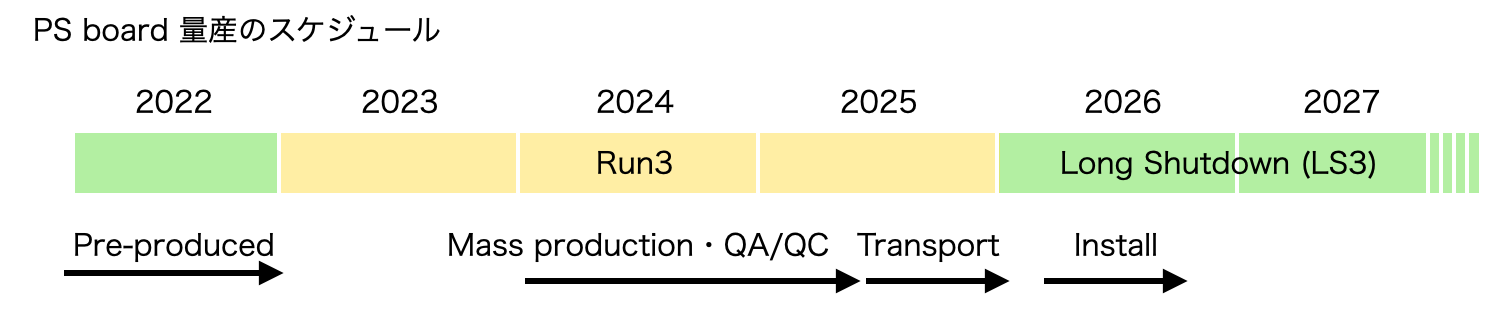
\includegraphics[width=16cm]{fig/QAQC/PSBschedule.png}
\caption[PS board量産のスケジュール]{PS board量産のスケジュール。PS boardはこれまでに第一試作機、第二試作機を通したシステム開発が完了いる。2023年現在、プレ量産された各個体に対しての試験を進めている。2024年から1400枚の本量産が開始され2026年から実験室への設置が開始される。}
\label{PSBschedule}
\end{figure}

\newpage
\subsection{PS board上の素子}
\label{subsec_PSBelements}
QAQC試験ではエレクトロニクス上のすべての素子間の同通を網羅的に検証することが重要である。
PS boardに搭載されている素子や各素子間の配線を把握し、ハードウェアを試験するのに十分な試験セットアップおよび試験内容を考案した。

図\ref{PSBconcept}にPS boardのインターフェイスと搭載されている素子、各素子間の配線について述べる。

\begin{figure} 
\centering
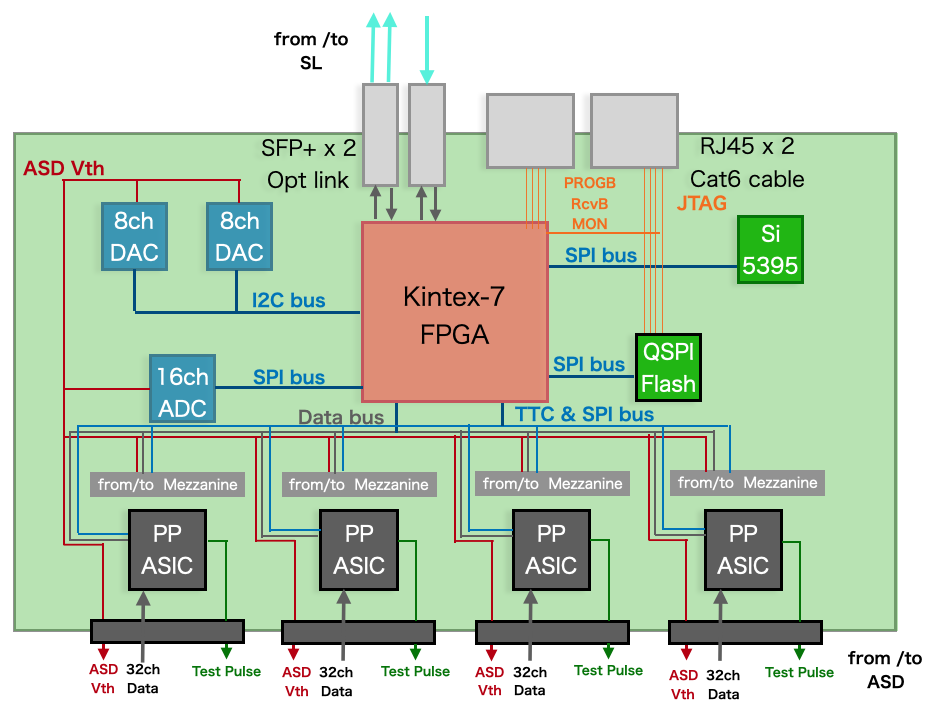
\includegraphics[width=16cm]{fig/QAQC/PSBoverall.png}
\caption[PSboardの全体像]{PS boardの全体像。PS boardに搭載されている各素子とその間の配線を示している。PS boardはSLと光ケーブル、JATHubとCat6ケーブルで接続される。PS board FPGAとDAC、ADC、Si5395、QSPI、PPASICはI2CまたはSPIバスで接続される。DACからアナログ信号として供給される閾値電圧は8台のASDボードとモニター用のADCに分配される。FPGAはPPASICにTTC信号を送信し、ヒット信号を受信する。1つのPPASICは2台のASDボードと接続されテストパルス信号を送信し、それぞれから8チャンネル分のヒットデータを受信する。}
\label{PSBconcept}
\end{figure}

\vskip0.5\baselineskip

\subsubsection{光ケーブル経由でのSLとの通信 } \par
PS boardは高速光シリアルリンクを介してSLと通信する。PS boardからの送信用として2リンク、受信用としてRX1リンク接続される。各リンクのラインレートは160bitのデータを40 MHzで、8B/10Bプロトコルに載せて送るので8Gbpsとなる。受信した光信号はSFP+モジュール内で電気信号へと変換され、FPGAに搭載されている高速シリアル通信対応のトランシーバーの一種である7シリーズGTXトランシーバーで受信される。PS boardからSLへは1枚のPS boardが担当する256チャンネル分のヒットデータが送られる。SLからPS boardへはコントロール信号が送信され、PS board FPGA上のレジスタ操作やPS board上の各素子の制御を行う。またTTC信号もコントロール信号に乗せられてPS boardに分配される。PS boardはシリアルデータからLHCバンチ交差クロックを再構成して動作クロックとして使用する。以下にPS board FPGAを介して制御される素子の一覧を示す。
\vskip0.5\baselineskip

\begin{enumerate}
    \item \texttt{QSPIフラッシュメモリー :} QSPIフラッシュモリーはPS board FPGAを中継としてSLからSPI線をビットバンギングすることで制御される。QSPIフラッシュメモリーにはPPASICやDACの制御用パラメーターが保存される。PS boardに電源が投入されるとFPGAは自らこのパラメーターを読み出し、PPASICとDACに分配する(自立型制御機構)。
    \vskip0.5\baselineskip

    \item \texttt{PPASIC :} PS board FPGA はQSPIフラッシュメモリーに書き込まれたPPASIC制御用パラメーターを読み出し、SPIプロトコルでPPASICをビットバンギングすることでPPASICを制御する。PPASICはASDから送られるヒット信号のデジタル化を担当しており、ヒット信号に対するディレイの大きさやBCIDゲートの幅などが決定される。その他にもPS board FPGAはTTC信号やテストパルストリガー信号をPPASICに送信し、PPASICからヒットデータを受け取る。
    \vskip0.5\baselineskip        

    \item \texttt{DAC :} PS board FPGA はQSPIフラッシュメモリーに書き込まれたDAC制御用パラメーターを読み出し、I2CプロトコルでDACをビットバンギングすることでPPASICを制御する。ASDに印加されるアナログの閾値電圧やその極性がこれにより決められる。
    \vskip0.5\baselineskip

    \item  \texttt{ADC :} PS board FPGA はSPI プロトコルを介して ADC をから電圧値を読み出す。ADCはDACからASDに印加される閾値電圧をモニターしており、FPGAから読み出されたADCの値はSLへと送信される。
    \vskip0.5\baselineskip

    \item \texttt{Si5395 :} PS board FPGA はSPIプロトコルを介してSi5395の制御を行う。Si5395制御用パラメーターはFPGA内のBRAMに格納されており、自立型制御機構のシークエンスの中でSI5395へのパラメーターが分配される。PS board FPGA内部で再構成されたLHCバンチ交差クロックはSi5395にてジッターの低減が行われ、FPGAやGTXトランシーバーへと分配される。
    \vskip0.5\baselineskip
\end{enumerate}

\subsubsection{Cat6ケーブル経由でのJATHubとの通信 :}\par
 PS boardは2本のCat6ケーブルを介してJATHubと通信する。一本のCat 6ケーブルには4線のLVDS線バンドルされており、それぞれ以下の3つの役割が割り当てられている。

\begin{enumerate}
    \item \texttt{JTAG線 :} 一本のCat 6ケーブルはJTAGプロトコルでのビットバンギング用に定義されておりJTAG線と呼ぶ。PS boardに搭載されているFPGAは内部の論理回路を何度でも書き直すことができる。しかし、一般にFPGAへ論理回路を書き込むには\footnote{ファームウェアを書くともいう}、書き込み用アプリケーションが走るホストPCをFPGAの近くまで持っていき、JTAG4線用のCopperケーブルでホストPCとFPGAを接続させる必要がある。PS boardはTGC検出器上に設置されており、実質的にそのようなアクセスはできない。そこで遠隔からのファームウェア書き込みの中継点として、JATHubが機能する。JATHubのメインドライバーであるZynq SoCのPS領域にはLinuxが起動してあり、PS boardとCopperケーブルで接続することでボード上のLinuxを起点にJTAG線をドライブすることができる。
    \vskip0.5\baselineskip


    \item \texttt{Recovery線 :} もう一本のCat 6ケーブルのうちRcvB線、PROGB線の2線はリカバリー手続きに使用される。一般に放射線の影響によりFGPA内部のレジスターの値がフリップする現象をSingle Event Upset(SEU)という。通常PS board上のFPGAで一つのSEUが発生した場合、Xilinxが提供するSoft Error Migration(SEM)によりこのレジスターの値は自己回復される。しかし、隣接する2つ以上のレジスターが同時にSEUを起こした場合にはSEMでは修復出来ず、回復不可能な状態となる。JATHubはRcvB線をモニターしこの自己回復不可能なSEU事象を発見し、PROGB線を通してファームウェアのリセット信号を送信する。リカバリー手続きの概要を図\ref{JATHubsem}に示す。
    \vskip0.5\baselineskip
    \begin{figure} 
    \centering
    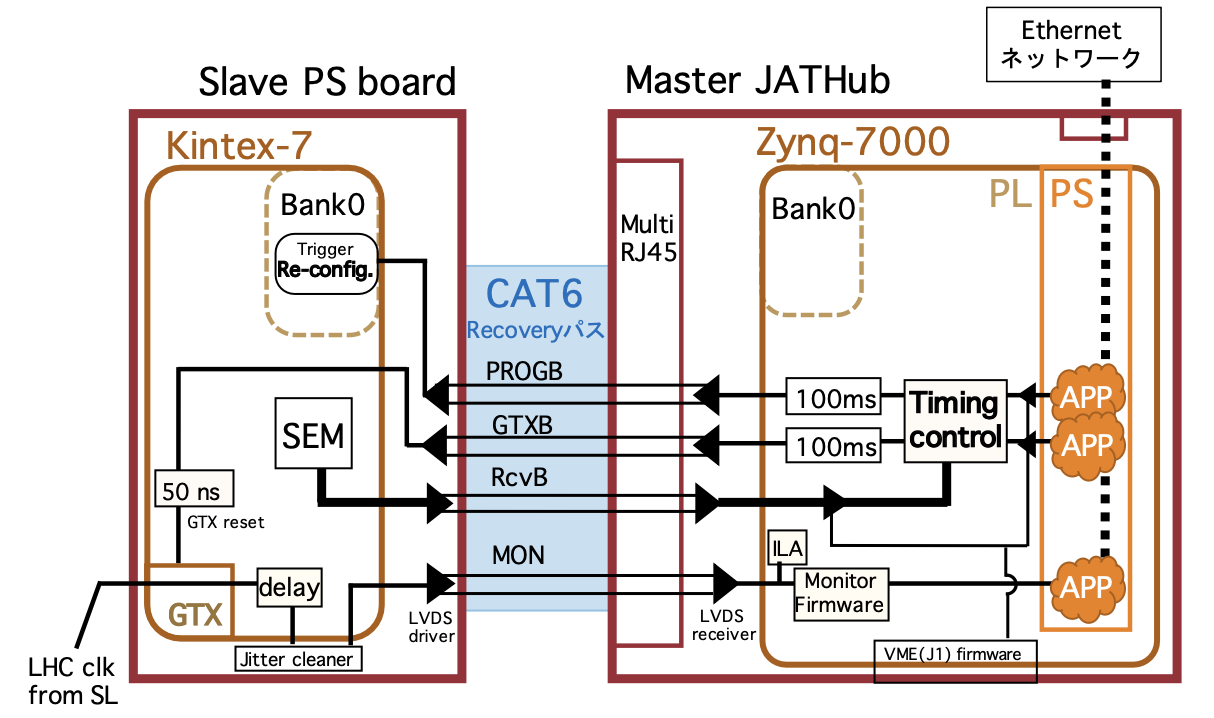
\includegraphics[width=16cm]{fig/QAQC/JATHubsem.png}
    \caption[JATHubによるリカバリー手続き]{JATHubによるリカバリー手続きの概念図。PS boardに自己修復不可能なSEU事象が発生した場合、RcvB線を通じてJATHubに救難信号が発出される。JATHubはPROBG線をアサートすることでPS board FPGAのリセットを命ずる。}
    \label{JATHubsem}
    \end{figure}
    
    \item \texttt{MON線 :} 残る1線はMON線として定義される。PS boardで再構成したLHCバンチ交差クロックをMON線を通じてJATHubへ送信し、JATHubに接続される11台のPS board間の相対的な位相差を測定するのに利用される。
    \vskip0.5\baselineskip
\end{enumerate}

\subsection{QAQC試験の設計}
\label{subsec_QAQCdesign}
\ref{subsec_PSBelements}節で述べたすべてのインターフェイスと搭載された素子を網羅的に試験可能なセットアップとしてPS baord 1台に対してJATHub1台を利用する図\ref{PSBtestdesign}の試験システムを考案した。

\begin{figure} 
\centering
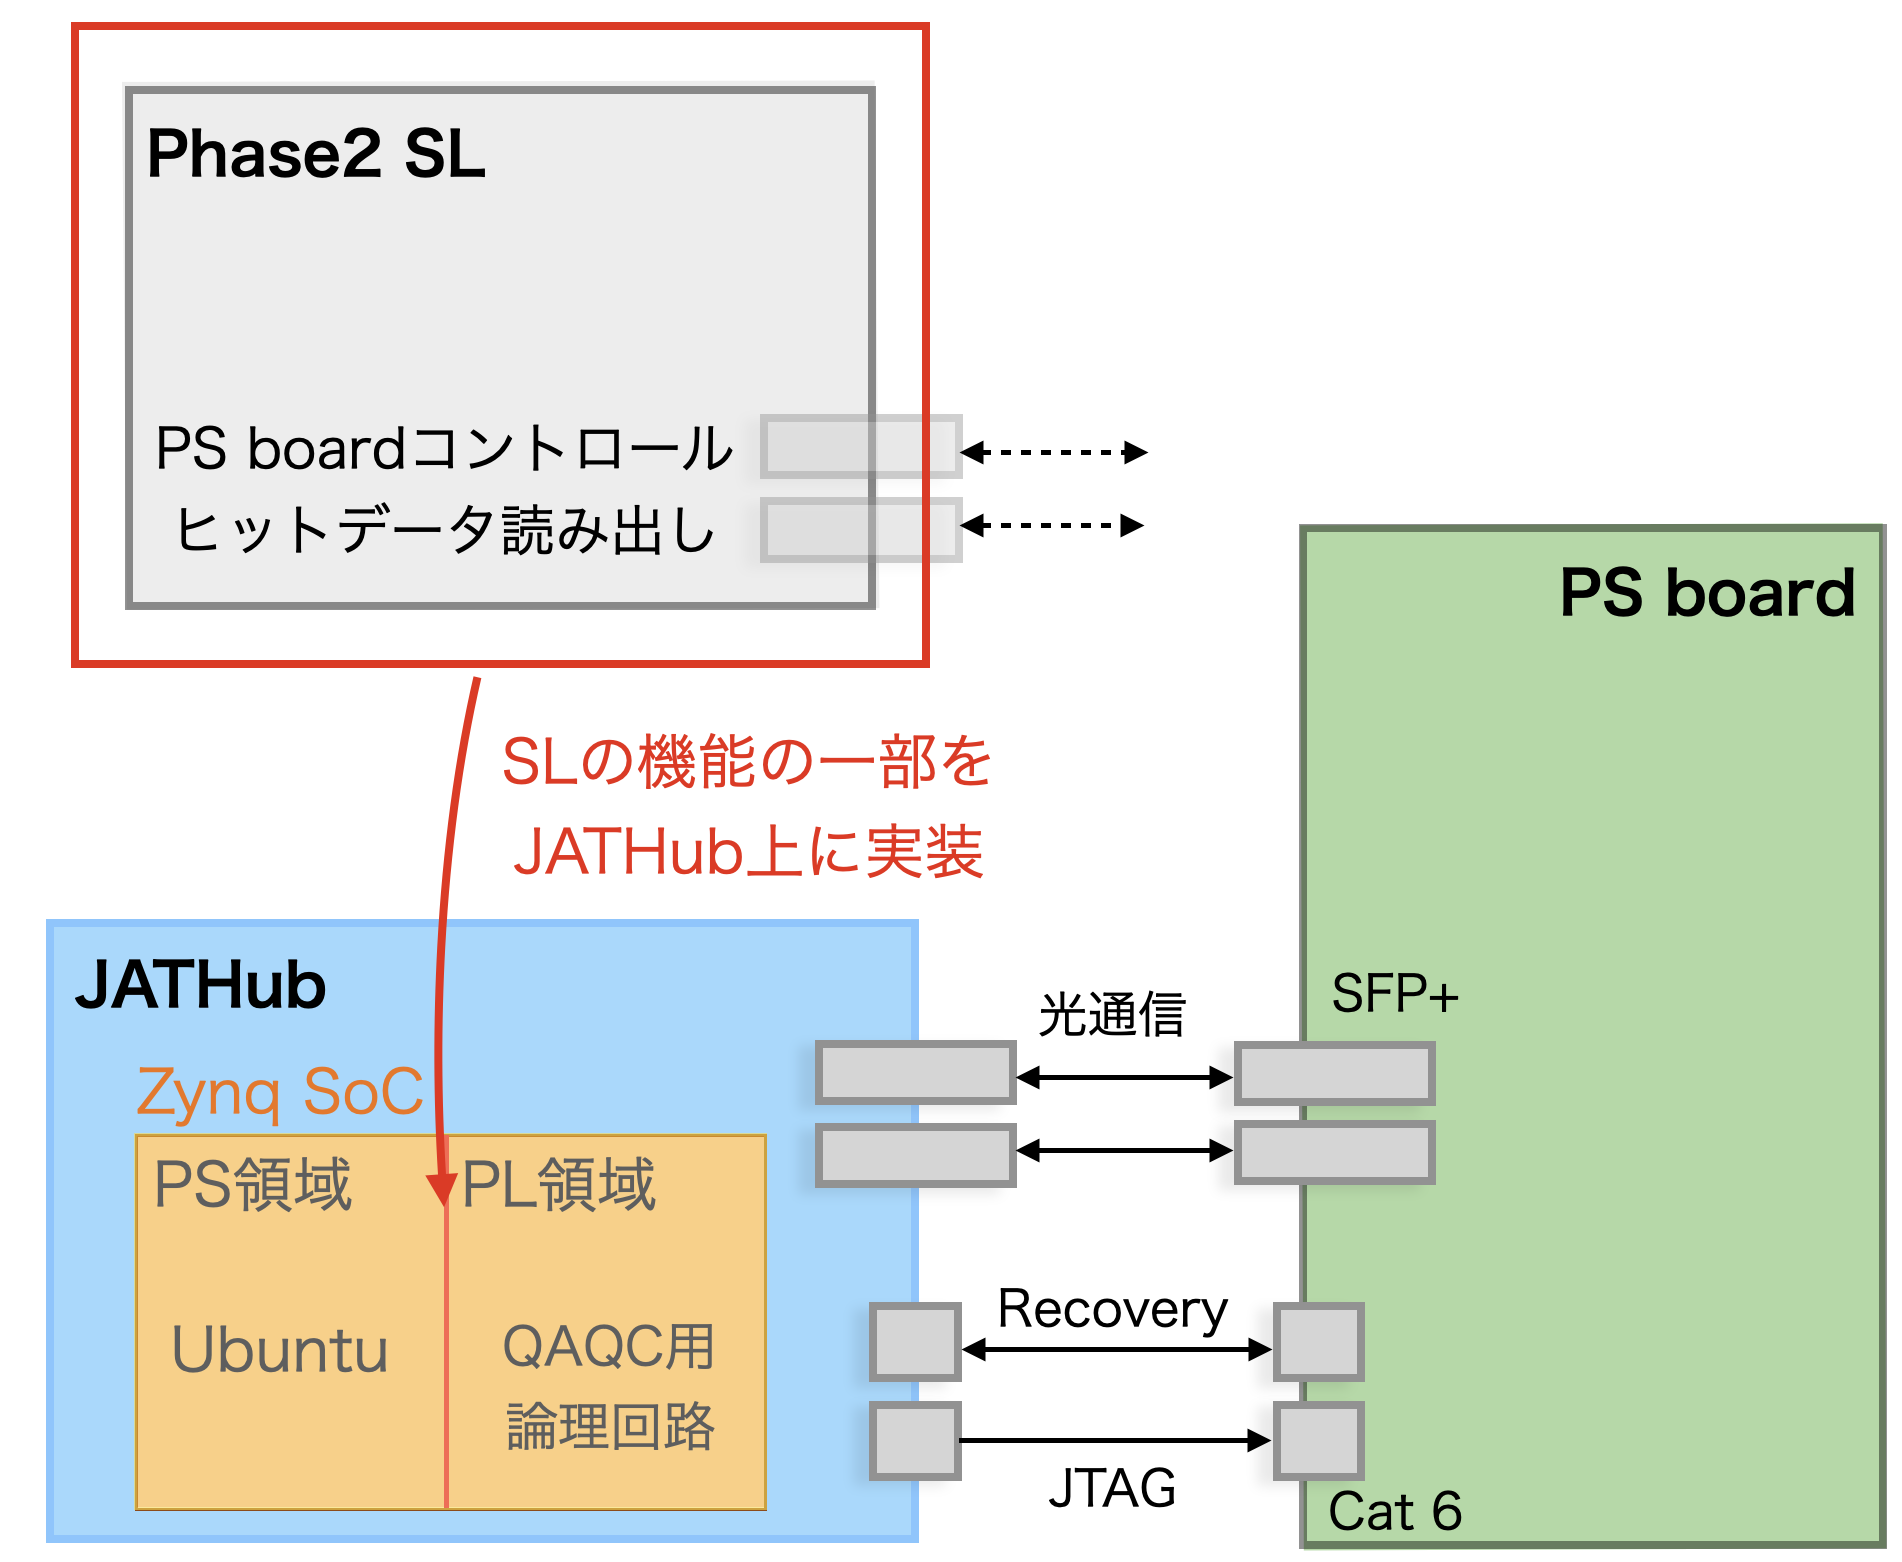
\includegraphics[width=16cm]{fig/QAQC/PSBtestdesign.png}
\caption[PS board QAQC試験セットアップの概念図]{PS board QAQC試験セットアップの概念図}
\label{PSBtestdesign}
\end{figure}

このシステムではPS boardの試験にJATHub1台のみを利用する。PS boardには試験用のファームウェアなどは用意せず、TGC DAQシステムとして実際に使うファームウェアを用いる。JATHubのメインドライバーであるZynq SoCのPS領域には汎用的なOSであるUbuntuを起動する。FPGA部分であるPL領域には試験用に新しくファームウェアを開発する。QAQC試験のマスターとして動作させるJATHubを以降ではQAQC用 JATHubと呼ぶ。JATHubとPS boardは2本のCat 6ケーブルに加え2リンクの光ケーブルで接続する。QAQC用JATHubのFPGAではGTXトランシーバーを実装し、SLとPS board間の通信と完全に等価な8 Gbpsのシリアル通信を行う。これによりQAQC用JATHubはSLが行うPS boardのコントロールマスター、ヒット信号のレシーバーとしての役割を代替する。PS boardの有するインターフェイスを網羅し十分な試験を実現することができる。このシステムではSLを利用せずJATHub1台のみを用いたことでコンパクトなセットアップを実現している。JATHubはデスクトップでも給電することが可能であり、場所を選ばない汎用的な試験システムとなっている。\par

QAQC用JATHubのファームウェア開発にあたり、\ref{subsec_PSBelements}節で挙げたPS board上のすべての素子とその間の導通を検証できる必要十分な試験として、ASDテストパルス試験とJTAG/Recovery/Clock monitor試験をベンチマークとして設定した。

\subsubsection{ASDテストパルス試験}
\label{subsubsec_testpulse}
\textbf{概要}\par
ASDテストパルスとはPPASICからASDに発せされる試験用電荷のことである。
図\ref{PSBasdtp}に示すようにASDより上流のデータ処理パスのデバッグに使われる。TGCエレクトロニクス系ではSLを起点にテストパルスの駆動を司るテストパルストリガー信号(TPT)が発行され、PS board FPGA、PPASICへと伝達される。PPASICにおけるテストパルスジェネレーター(Test Pulse Generator,TPG)の回路図を図\ref{PSBtpg}に示す。テストパルスジェネレーターはTPT信号をトリガーに、参照クロックである40 MHzクロックの立ち上がりと同期した差動の矩形波(テストパルス)をASDに送信する。テストパルスはASD、PPASIC、PS board FPGAからなるフロントエンドエレクトロニクスによる処理を経て、ヒット信号としてSLに送信される。SLで期待したBCにヒット信号が得られることを確認することでSLからASDまでのTDAQパスが固定レイテンシーで動作していることを確かめることができる。
\vskip0.5\baselineskip
\begin{figure} 
\centering
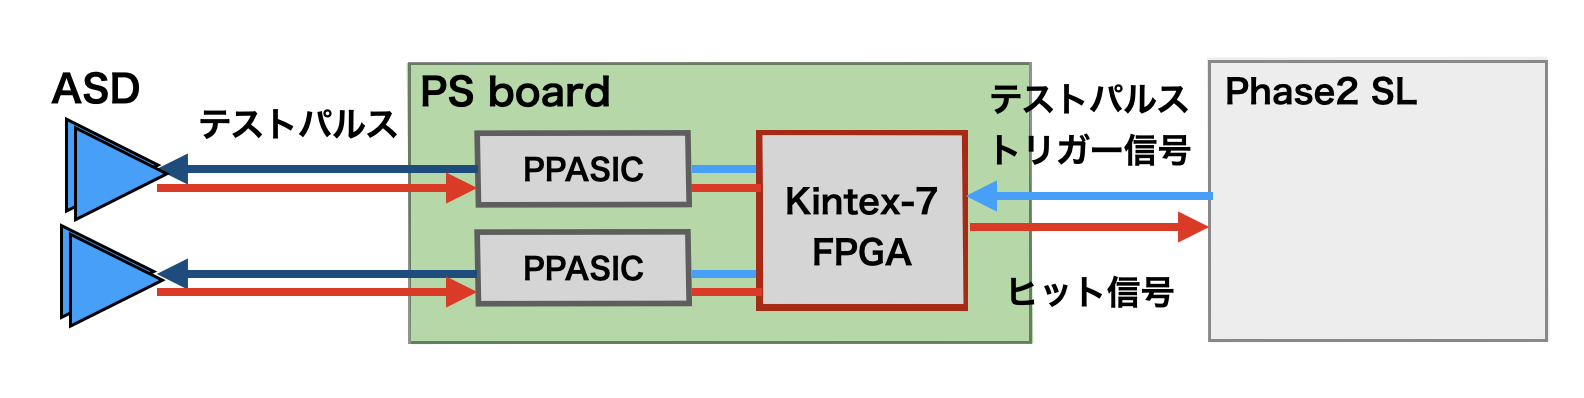
\includegraphics[width=16cm]{fig/QAQC/PSBasdtp.png}
\caption[ASDテストパルスの概念図]{ASDテストパルス機構の概念図。SLを起点にテストパルストリガー信号が駆動され、PS board FPGAを経由してPPASICに届けられる。PPASIC内のテストパルスジェネレーターはテストパルストリガー信号をトリガーに参照クロックの立ち上がりと同期した試験電荷をASDに送る。ASDで閾値電圧を信号はデジタル信号へ変換され、PPASIC、PS board FPGA、SLへとヒット信号が伝搬される。}
\label{PSBasdtp}
\end{figure}

\textbf{手順}\par
図\ref{QAQCasdtp}に示すようにQAQC試験ではQAQC用JATHubが試験のマスターとして、PS boardの制御、テストパルストリガーの駆動およびヒットデータの読み出しを行う。Zynq SoCのPL領域にPS board制御および読み出しのための回路を実装し、Ubuntu上のアプリケーションを起点に動作する。読み出し回路によりUbuntuに読み出されたヒットデータはローカルのSDカード上にテキストファイルとして保存する。以下に試験の手順を示す。

\begin{figure} 
\centering
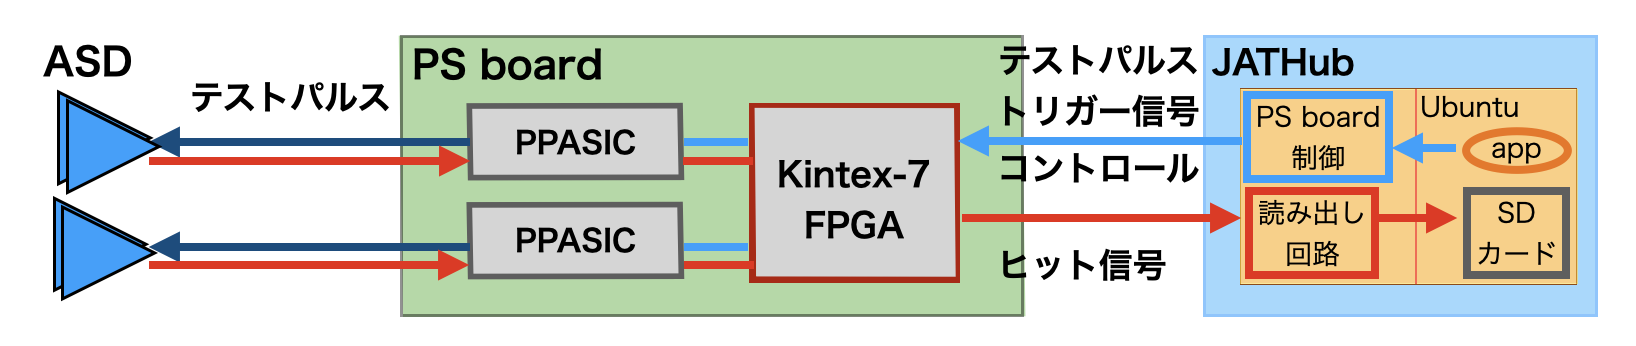
\includegraphics[width=16cm]{fig/QAQC/QAQCasdtp.png}
\caption[QAQC用JATHubを用いたASDテストパルス試験]{QAQC用JATHubを用いたASDテストパルス試験。QAQC用JATHubが試験のマスターとして、PS boardの制御、テストパルストリガーの駆動およびヒットデータの読み出しを行う。Zynq SoCのPL領域にPS board制御および読み出しのための回路を実装し、Ubuntu上のアプリケーションを起点に動作する。読み出し回路によりUbuntuに読み出されたヒットデータはローカルのSDカード上にテキストファイルとして保存する。}
\label{QAQCasdtp}
\end{figure}

\begin{enumerate}
    \item QAQC用JATHubをコントロールマスターとしてUbuntu上のアプリケーションを起点にPS board上の素子のコンフィギュレーションおよび設定値の監視を行う。具体的にはDACの閾値電圧、極性、PPASICの信号遅延、テストパルスの極性、テストパルスの波高、テストバルスの幅、BCIDゲート幅などのパラメーターを設定する。
    \vskip0.5\baselineskip

    \item QAQC用JATHubからテストパルストリガーを発行。光リンクに載せてPS board FGPAへ送信。
    \vskip0.5\baselineskip

    \item テストパルストリガーを発行してからヒット信号が返ってくるまでのレイテンシーをあらかじめ測定しておき、そのタイミングに合わせてヒットデータを読み出す。1台のPS boardが担う全256チャンネルでヒット信号が埋まっていることを確認する。
    \vskip0.5\baselineskip

    \item 2,3を約1万回繰り返し、固定レイテンシーでのDAQが長時間安定して動作することを確認する。
\end{enumerate}

\textbf{検証できる素子}\par
ASDテストパルス試験に関与する素子とパスを図\ref{QAQCasdtpelements}に示す。ASDテストパルスを期待通り動作させるにはPPASIC、DAC、Si5395に適したパラーメーターを分配し、ASD、PPASIC、PS board FPGA、光リンクが同期して動作する必要がある。この試験によりPS boardのJATHubとのインターフェイス以外のすべての機能を検証することができる。
\vskip0.5\baselineskip

\begin{figure} 
\centering
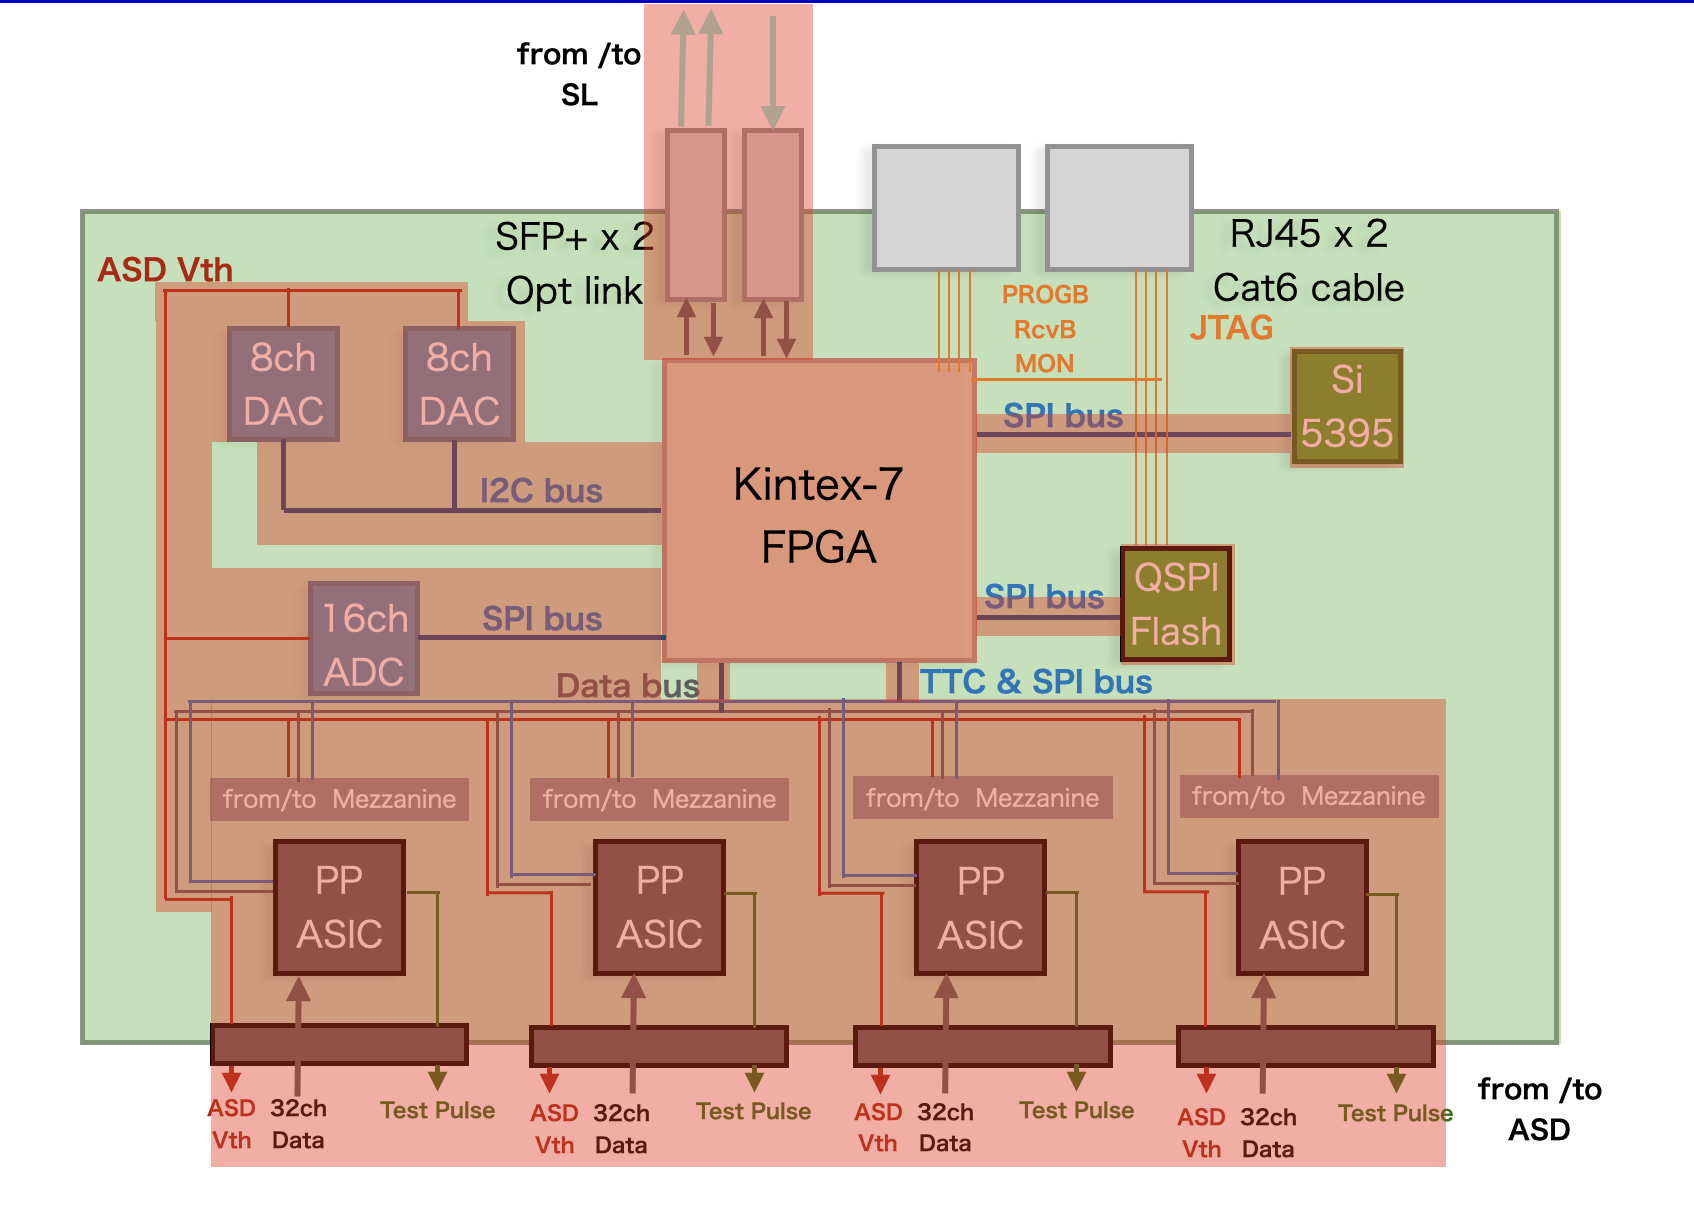
\includegraphics[width=16cm]{fig/QAQC/QAQCasdtpelements.png}
\caption[ASDテストパルス試験で検証できる素子]{ASDテストパルス試験で検証することができる素子、素子間の配線を赤枠で示す。}
\label{QAQCasdtpelements}
\end{figure}

\subsubsection{JTAG/Recovery/Clock試験}
\label{subsubsec_jtag}
JATHubがPS boardに対して行うJTAG線を介したファームウェアの書き込み、リカバリー手続き、クロック位相測定がすべての個体で動作することを試験する。これらの機能は先行研究で開発されており、それをQAQC用JATHubにも統合しUbuntuをメインドライバーとして実行することで試験する。

\begin{itemize}
    \item \textbf{JTAG試験}\par
    QAQC用JATHub上のUbuntuをドライバーとしてJTAG4線を操作しPS board のQSPIフラッシュメモリーにファームウェアを書き込む。SDカードに保存したSerial Vector Format (SVF)ファイルと呼ばれるASCIIファイルを元にJTAG4線を操作する。
    \vskip0.5\baselineskip

    \item \textbf{リカバリー試験}\par
    %図作る
    リカバリー試験の概念図を図\ref{QAQCrecovery}に示す。PS boardにはSEMを模してRcvB線をlowにするためのレジスターが用意されている。QAQC用JATHubからそのレジスターを操作することで仮想的に救難信号を発出する。救難信号を受けたらQAQC用JATHubからPROGB線をアサートし、PS boardがリセットされることを確認する。
    \vskip0.5\baselineskip
    
    \item \textbf{クロック試験位相測定}\par
    MON線経由で送られる40 MHzクロックの位相をJAThub内の水晶発振器から生成した40 MHzクロックを参照クロックにして測定する。システムの概念図を図\ref{JATHubclockmeasure}\cite{mt_atanaka}に示す。Vivadoで提供されるClocking WizardというIPを用いて参照クロックを1/56 ns刻みで位相をシフトすることができる。この機能を用いて参照クロックをシフトさせながら、参照クロックの立ち上がりでPS boardからのクロックをサンプリングすることでクロックの位相を測定する。
    \vskip0.5\baselineskip
 
\end{itemize}



\begin{figure} 
\centering
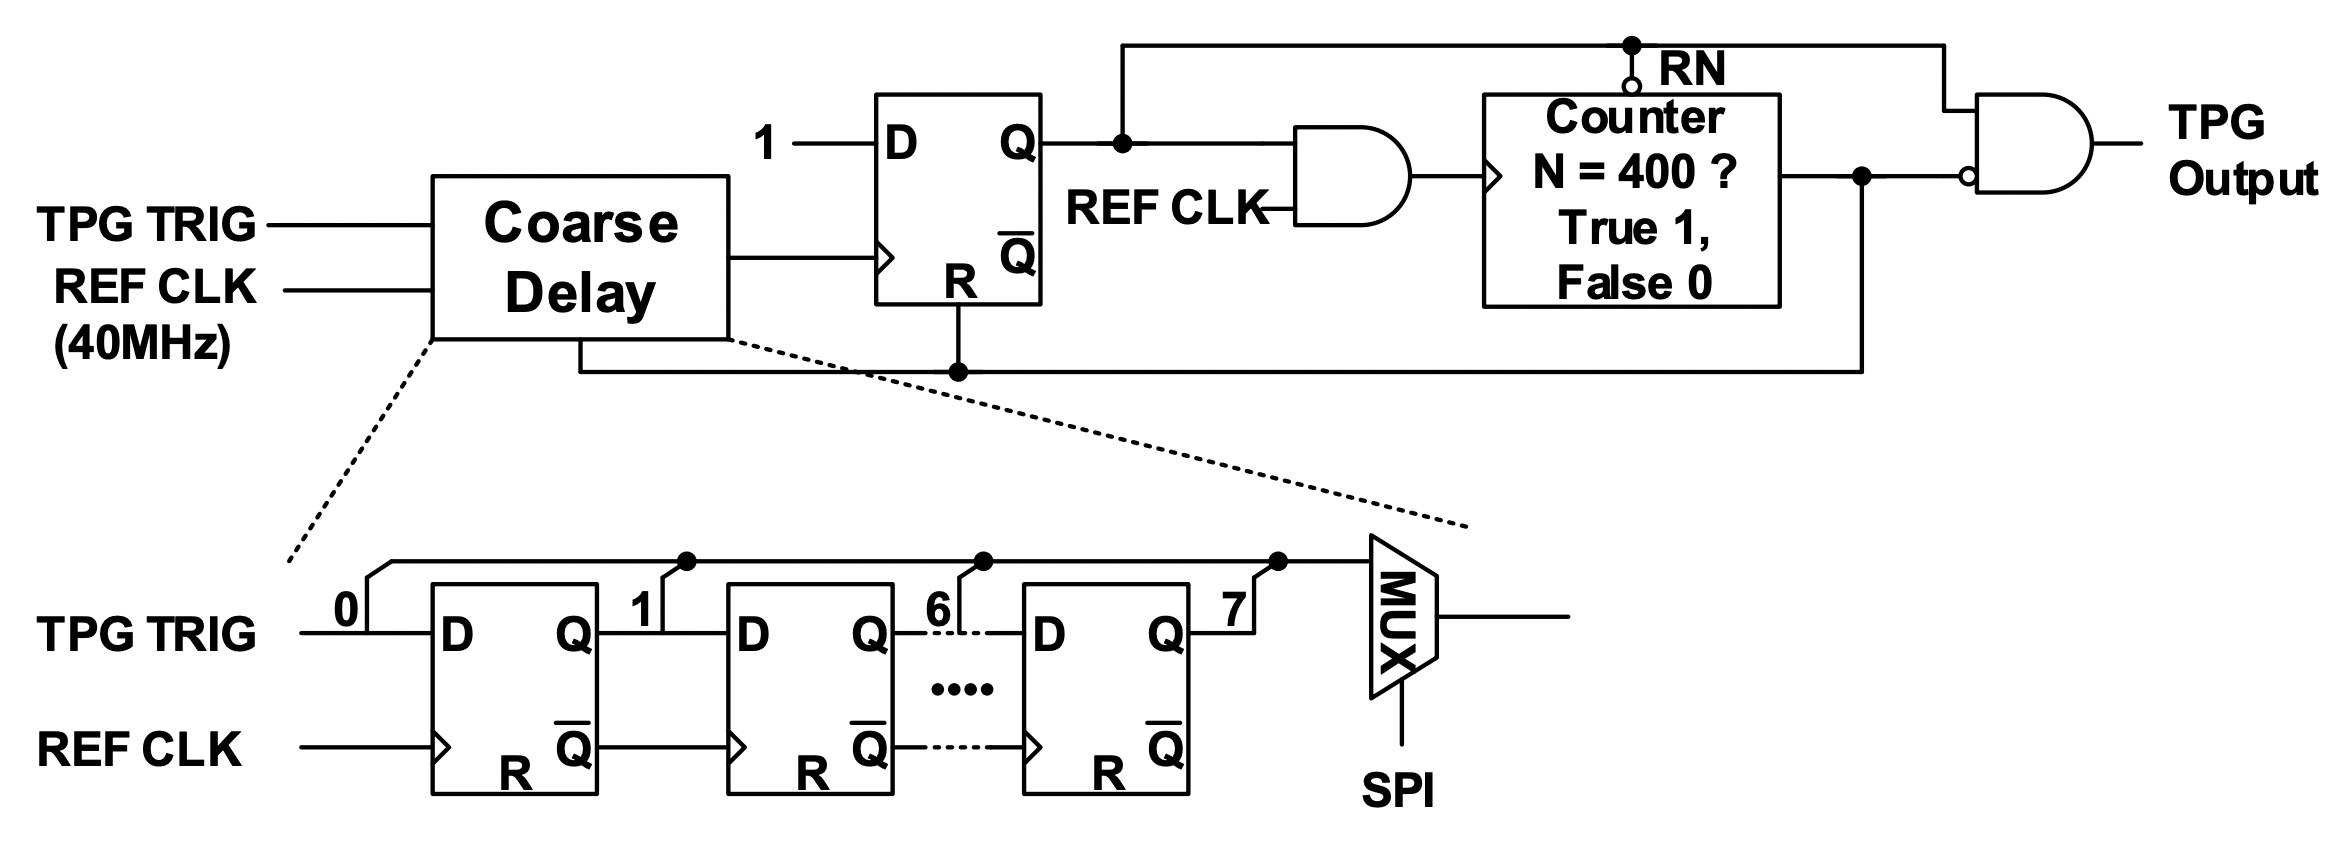
\includegraphics[width=16cm]{fig/QAQC/PSBtpg.png}
\caption[テストパルスジェネレーターの回路図]{テストパルスジェネレーターの回路図。PS board FPGAからTRIG信号を受け取り、参照クロックである40 MHzクロックの立ち上がりに同期してASDに対して差動の矩形波を送信する。矩形波の幅や高さはFPGAから設定可能なパラメーターである。}
\label{PSBtpg}
\end{figure}

\section{コンパクトDAQシステムの機能実装}
本節では\ref{subsec_QAQCdesign}節で考案した試験を実現するために、QAQC用JATHubに実装した機能について述べる。まずQAQC用JATHubに存在する複数の物理レイヤーをまたぐインフラ部分の設計について述べる。次に論理回路部分に実装した機能について述べる。

\subsection{QAQC用JATHubインフラ部分の実装}
\label{subsec_infra}
まずはQAQC用JATHubにおける物理階層とその階層をまたぐインターフェイスの実装について述べる。
図\ref{JAThubinfra}にシステムの全体像を示す。このQAQC用JATHubはZynq MPSoC上のPS部、PL部で構成される。ローカルPCからネットワーク経由でPS部分を操作し、PL部分からPS boardの制御信号を送る。Zynq MPSoCのPS部分には標準的なLinux OSであるUbuntuを起動する。Ubuntuから論理回路部分の操作はXilinxが提供するIPの一種であるAXI General Pupose IO(GPIO)を利用する。FPGAには固定レイテンシーでのGTXトランシーバーを実装し、高速光通信を介して通信を行う。PL内の読み出し回路からUbuntuへのデータ読み出しにはAXI GPIOを応用した自作調停回路を実装した。

\begin{figure} 
\centering
\includegraphics[width=16cm]{fig/QAQC/JAThubinfra.png}
\caption[QAQC用JATHubのシステム全体像]{QAQC用JATHubのシステム全体像}
\label{JAThubinfra}
\end{figure}

\subsubsection{Zynq MPSoCにおけるUbuntuの起動}
\label{subsubsec_ubuntu}
\vskip0.5\baselineskip
Zynq MPSoCのPS部分には標準的なLinux OSであるUbuntuを起動する。Ubuntuを利用することでネットワークの設定やQAQC用JATHub内部でのアプリケーション開発を容易に行うことができる。\par

Zynq組み込みデザインの開発には64bit Ubuntu 18.04.6を使用した。Xilinx社が提供する”Vivado 2020.2”を利用してZynq PL部に構築する自作論理回路の開発やPS部のIO設計を行った。Vivadoで開発した論理回路は最終的にBitstreamファイルと呼ばれるバイナリーファイルに記述される。またZynq PS 部で走るLinuxの設定はXilinx社が提供するクロスコンパイラー”petalinux 2020.2”を利用した。PetalinuxではVivadoで生成したHDFを元にデバイスツリーやRoot File System(rootfs)を設定することで、Zynqの起動に必要なブートファイルを作成することができる。\par
QAQC用JATHubではUbuntuの起動にSDカードを利用する。Zynqの起動に必要なブートファイルとUbuntuのルートファイルシステムをれぞれ異なるパーティションに展開する。図\ref{JATHubboot}にZynq上でのUbuntu起動の流れを示す\cite{mt_okazaki}。JATHubに電源を投入すると以下のシークエンスでUbuntuが起動する。

\begin{figure} 
\centering
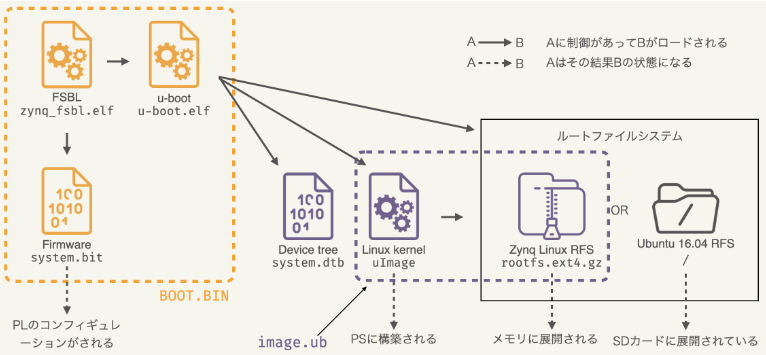
\includegraphics[width=16cm]{fig/QAQC/JATHubboot.png}
\caption[Ubuntuの起動シークエンス]{Ubuntuの起動シークエンス}
\label{JATHubboot}
\end{figure}

\begin{enumerate}
    \item First Stage Boot Loader(FSBL)がロードされる
    \item ファームウェアのビットストリームがSoCのPL部に書き込まれる
    \item LinuxカーネルやOSを起動するためのブートローダーであるu-bootがロードされ、制御が移行される。
    \item u-boot 制御下でデバイスのハードウェア情報を記述したデバイスツリーがロードされる。
    \item u-boot 制御下でLinux kernelがロードされPS部に構築される。
    \item u-boot 制御下でLinux kernelがロードされPS部に構築される。
    \item 制御がLinuxカーネルに移行されLinuxが起動する。
\end{enumerate}

\subsubsection{LANケーブル経由のネットワーク通信}
\label{subsubsec_network}
\vskip0.5\baselineskip
QAQC試験で用いるJATHub試作1号機は2通りの方法でEthernet通信を行うことができる。それぞれの方法は先行研究で開発されている(図\ref{JATHubnetwork}\cite{mt_atanaka})。1つ目はボード上に搭載されたPHY chipでEthernet信号を処理する方法で、LAN(Copper)ケーブルとRJ45コネクターを用いて通信することができる。2つ目はPL領域でPHYの信号処理を行う方法で、光ケーブルとSFPコネクターを用いて通信する。QAQC用JATHubでは2リンクある光ケーブルはどちらもPS board との高速シリアル通信に利用するため、1つ目の方法を利用してネットワーク接続を行う。


\subsubsection{AXI GPIOを用いたPSからPLへのアクセス}
\label{subsubsec_axi}
PS領域からPL領域への通信は統一的にAXI General Purpose Input Output(GPIO)を介して行う。AXI GPIOによって接続されたPLのレジスタには固有の物理的アドレスが割り当てられる。割り当てられrた物理アドレスの例を図\ref{JATHuaddress}に示す。このアドレスはVivadoのAddress Mapで確認することができ、Address Editorにてユーザーが自由に変更することができる。
PS領域からこのレジスタへは少なくとも2通りの方法でアクセスすることができる。1つはUbuntuルートファイルシステム内の/dev/memが提供するキャラクターデバイスをアプリケーションから直接開く方法である。/dev/memを介したアクセスではUbuntuが扱うすべての物理アドレスに制限なくアクセスすることができるため、簡単に使用できる。一方、カーネル動作に必要なレジスタにもアクセスすることが可能なため、カーネル動作に必要なレジスタを意図せず書き換えてしまうことなどによりカーネルを壊す危険性がある。2つ目の方法特定のAXI GPIOレジスタをUser space I/O(UIO)としてデバイスツリーに登録し、アプリケーションからUIOドライバーを介してアクセスする方法である。この方法ではUIOに登録したアドレス以外へのアクセスは禁止されるためカーネルを壊す危険性がなくなる。また割り込み処理ができるという利点もある。コントロールパスにおいてはより実装が簡単な/dev/memを直接用いる方法をとっている。
\vskip0.5\baselineskip

\begin{figure} 
\centering
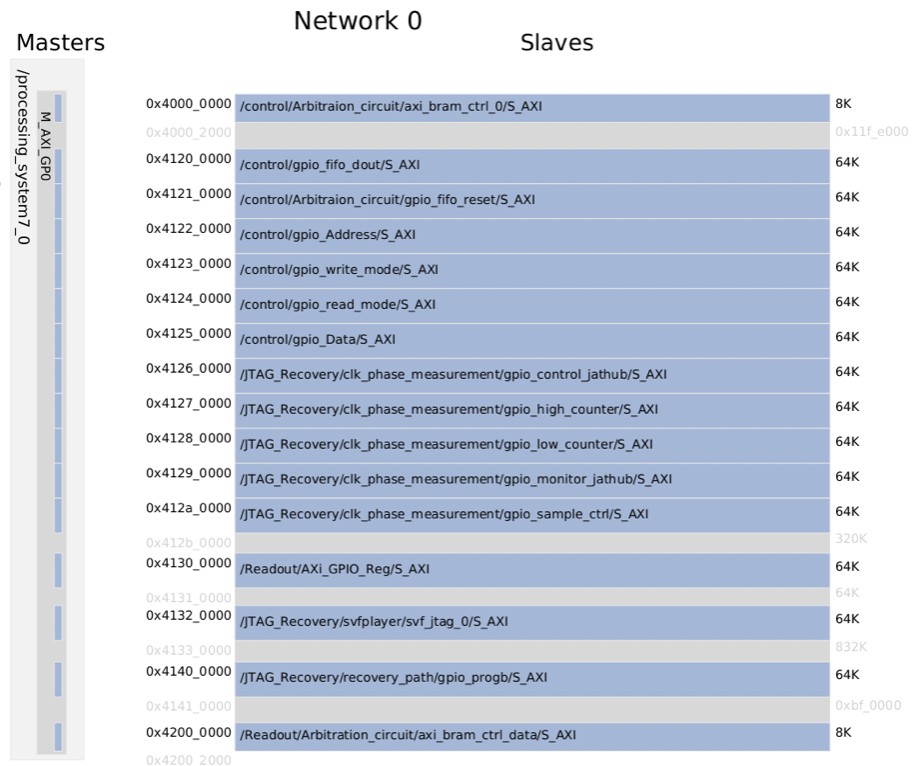
\includegraphics[width=10cm]{fig/QAQC/JATHubaddress.png}
\caption[アドレスマップ]{JAThub PL領域に割り当てられたアドレスマップ。各AXI GPIOレジスタには固有の物理アドレスが割り当てられる。}
\label{JATHuaddress}
\end{figure}

\subsubsection{固定位相光シリアル通信のためのGTXトランシーバーの実装}
\label{subsubsec_gtx}
\ref{subsec_PSBelements}節で述べたようにSLとPS boardの間では光リンクを介した固定位相のクロック分配が行われる。LHCバンチ交差クロックとPS baordで再構成されるクロックの位相関係が変化しないことはPP ASICで適切なBCIDをするのに不可欠な要請である。PS boardのこの機能を検証するため、QAQC用JATHubを用いたASDテストパルス試験においても固定位相でのDAQが実現できていることを確認する。そこで先行研究で開発された固定位相でのクロック分配のためのGTXトランシーバーを本システムにも組み込んだ。図\ref{JATHubgtx}にGTX実装の概要を示す。
\vskip0.5\baselineskip

\begin{figure} 
\centering
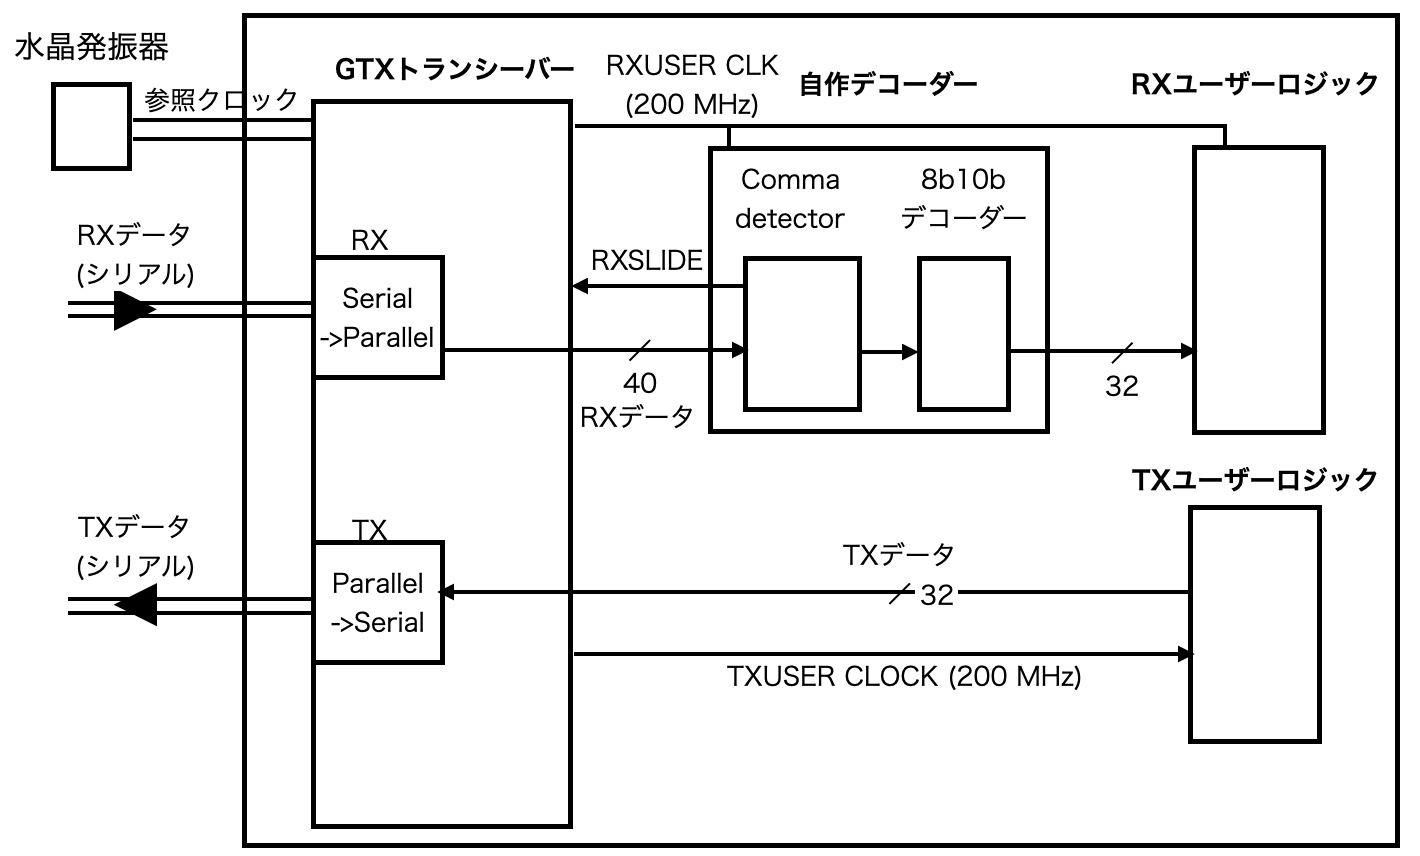
\includegraphics[width=16cm]{fig/QAQC/JATHubgtx.png}
\caption[QAQC用JATHubにおけるGTXトランシーバーの概要]{QAQC用JATHubにおけるGTXトランシーバーの概要}
\label{JATHubgtx}
\end{figure}


\textbf{TXロジック}
\vskip0.5\baselineskip
GTXトランシーバー部分はJATHub内部の水晶発振器から生成される200 MHzクロックを参照クロックとして利用する。\ref{subsec_PSBelements}節で述べたようにQAQC用JATHubとPS baord間の1リンクのラインレートは40 MHz x 160 bit x 10/8 = 8 である Gbpsである。TXでは200 MHzの参照クロックをそのままユーザーロジックの動作クロックとして利用する。200 MHzおきに32bitのパラレルデータ(1 ワードと呼ぶ)をGTXトランシーバーに送信し、GTXトランシーバー内で8b/10bのプロトコルで40 bitのパラレルデータへとエンコードした後、シリアルデータへと変換する。生成されたシリアルデータは参照クロックをGTXトランシーバー内のPhase Locked Loop(PLL)で冪倍して得られる4 Gbpsのクロックに乗せられ送信される。
\vskip0.5\baselineskip

\textbf{RXロジック}
RXロジック重要な役割を果たすのがRX Clock Data Recovery機構(CDR)とcomma detectorである。CDR機構とは受信したシリアルデータの立ち上がりまたは立ち下がりのタイミングに同期してクロックを再構成する機能で、受信データと位相関係を固定してクロックを再構成することができる。CDRで再構成された4 GHzクロックは1/20に分周され200 MHz RXユーザークロックが作られるが、1/20分周の過程で合計20種類の位相の不確定性が生じる。この中から特定の1つの位相を決めるために用意されているのがComma detectorである。commaデータとは送信側と受信側の間で事前に取り決められた10 bitの予約語で、本システムでは40 MHzに一回送信するよう決める。comma detectorはcommaデータが下位10bitにくるまでシリアルデータをシフトする機能である(図\ref{JATHubcomma})。40 MHzで送信される200 bitのシリアルデータから10bitの境界を定めることで再構成クロックの位相を一意に定めることができる。

\begin{figure} 
\centering
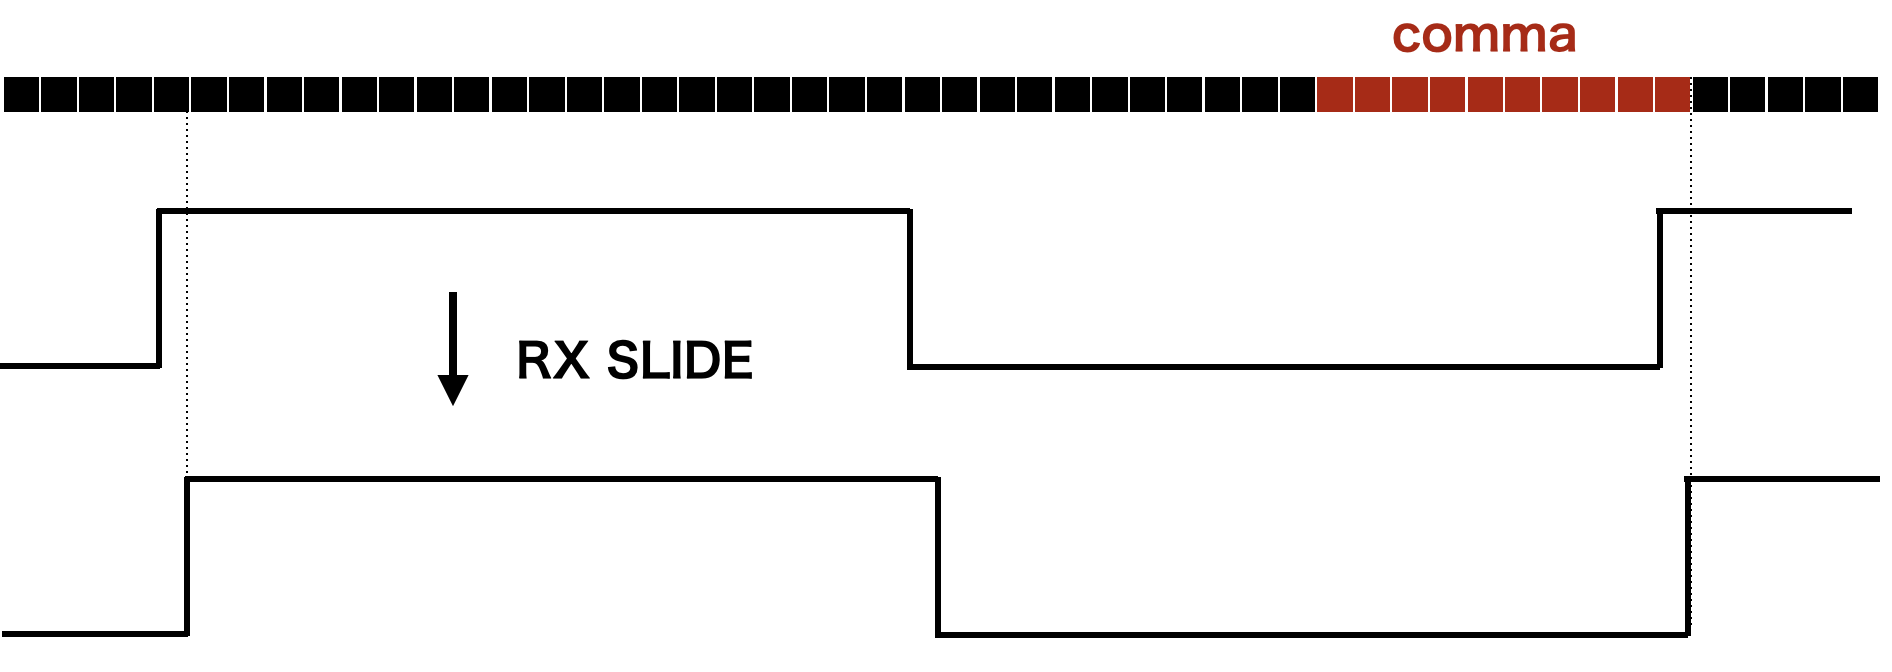
\includegraphics[width=16cm]{fig/QAQC/JATHubcomma.png}
\caption[comma detectorの概要]{comma detectorの概要}
\label{JATHubcomma}
\end{figure}
\vskip0.5\baselineskip


\subsubsection{PLからPSへのデータ読み出しシステム設計}
\label{subsubsec_readout}
Zynq FPGA内でのデータ転送はO(~10) MHzの高速クロックをもとに行われる。一般にPS部分をO(ns)で制御し、FPGAと同期してデータを読み出すことは困難である。そこでQAQC用JATHubでは異なる速度で動作する2つのプロセス間のデータ転送利用されるFirst In First Out(FIFO)メモリーを活用した自作調停回路を開発し、すべてのデータをもれなく読み出すことができる汎用読み出しシステムの実装を実装した。
図\ref{JATHubarbitor}に実装した読み出しシステムの概要を示す。

\begin{figure} 
\centering
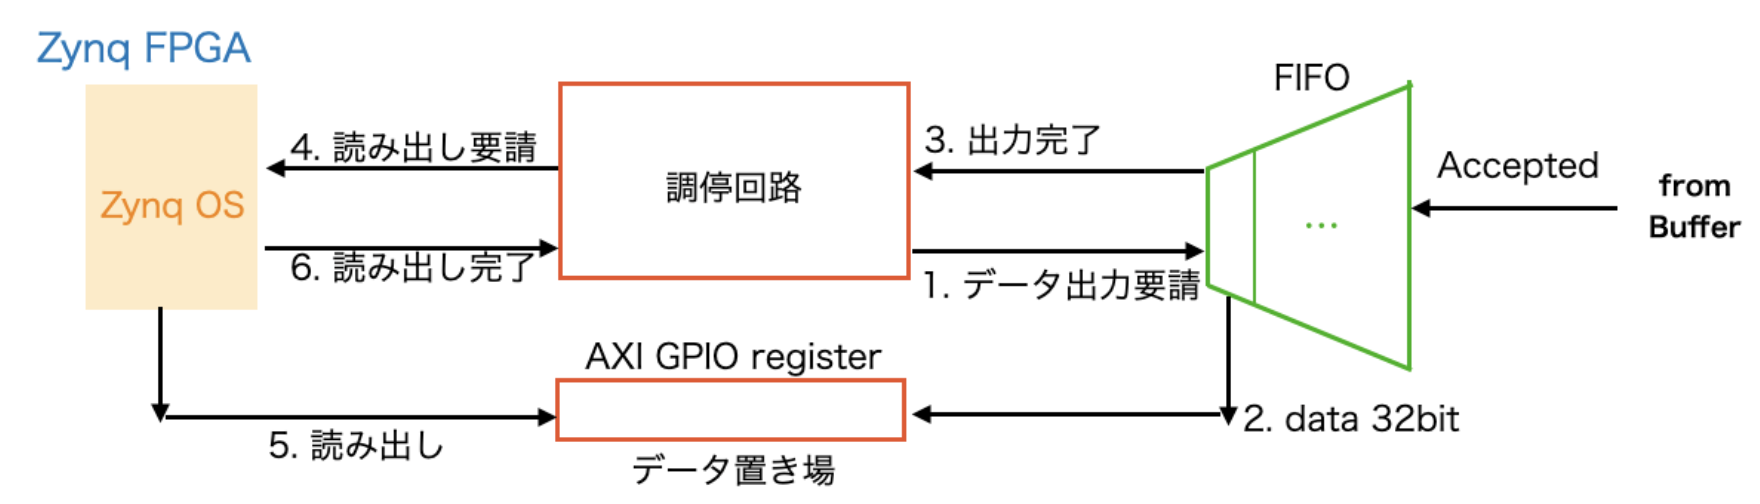
\includegraphics[width=16cm]{fig/QAQC/JATHubarbitator.png}
\caption[PLからPSでのデータ読み出しシステム概要]{PLからPSでのデータ読み出しシステム概要}
\label{JATHubarbitor}
\end{figure}

FPGA内からUbuntuに読み出したいデータはFPGA内の動作クロックに乗せられFIFOメモリーにダンプされる。UbuntuからFIFOに直接アクセスすることはできないため、両者のデータのやり取りにはAXI GPIOレジスタを利用する。
AXI GPIOレジスタにはFPGAからもUbuntuからも任意のタイミングでアクセスすることができる。そのためUbuntuがデータを読み出す前にFIFOがデータを書き換えると、そのデータはUbuntuから読み出されずロスすることになる。またFIFOがデータを書き換える前にUbuntuが2回読み出し動作を行うと、同じデータが重複して読み出される。全てのデータを漏れや重複なく読み出すため、FIFOとUbuntuがAXI GPIOレジスタにアクセスするタイミングを取り持つ調停回路を設置した。調停回路は1bitのフラグとステートマシンからなる。フラグはUbuntuとFIFO間の状況伝達に利用しており 0: FIFOからの書き込み待ち 1: Ubuntuからの読み出し待ちで定義する。調停回路で実現される読み出しシークエンスを\ref{JATHubarbitation}で示す。
\begin{figure} 
\centering
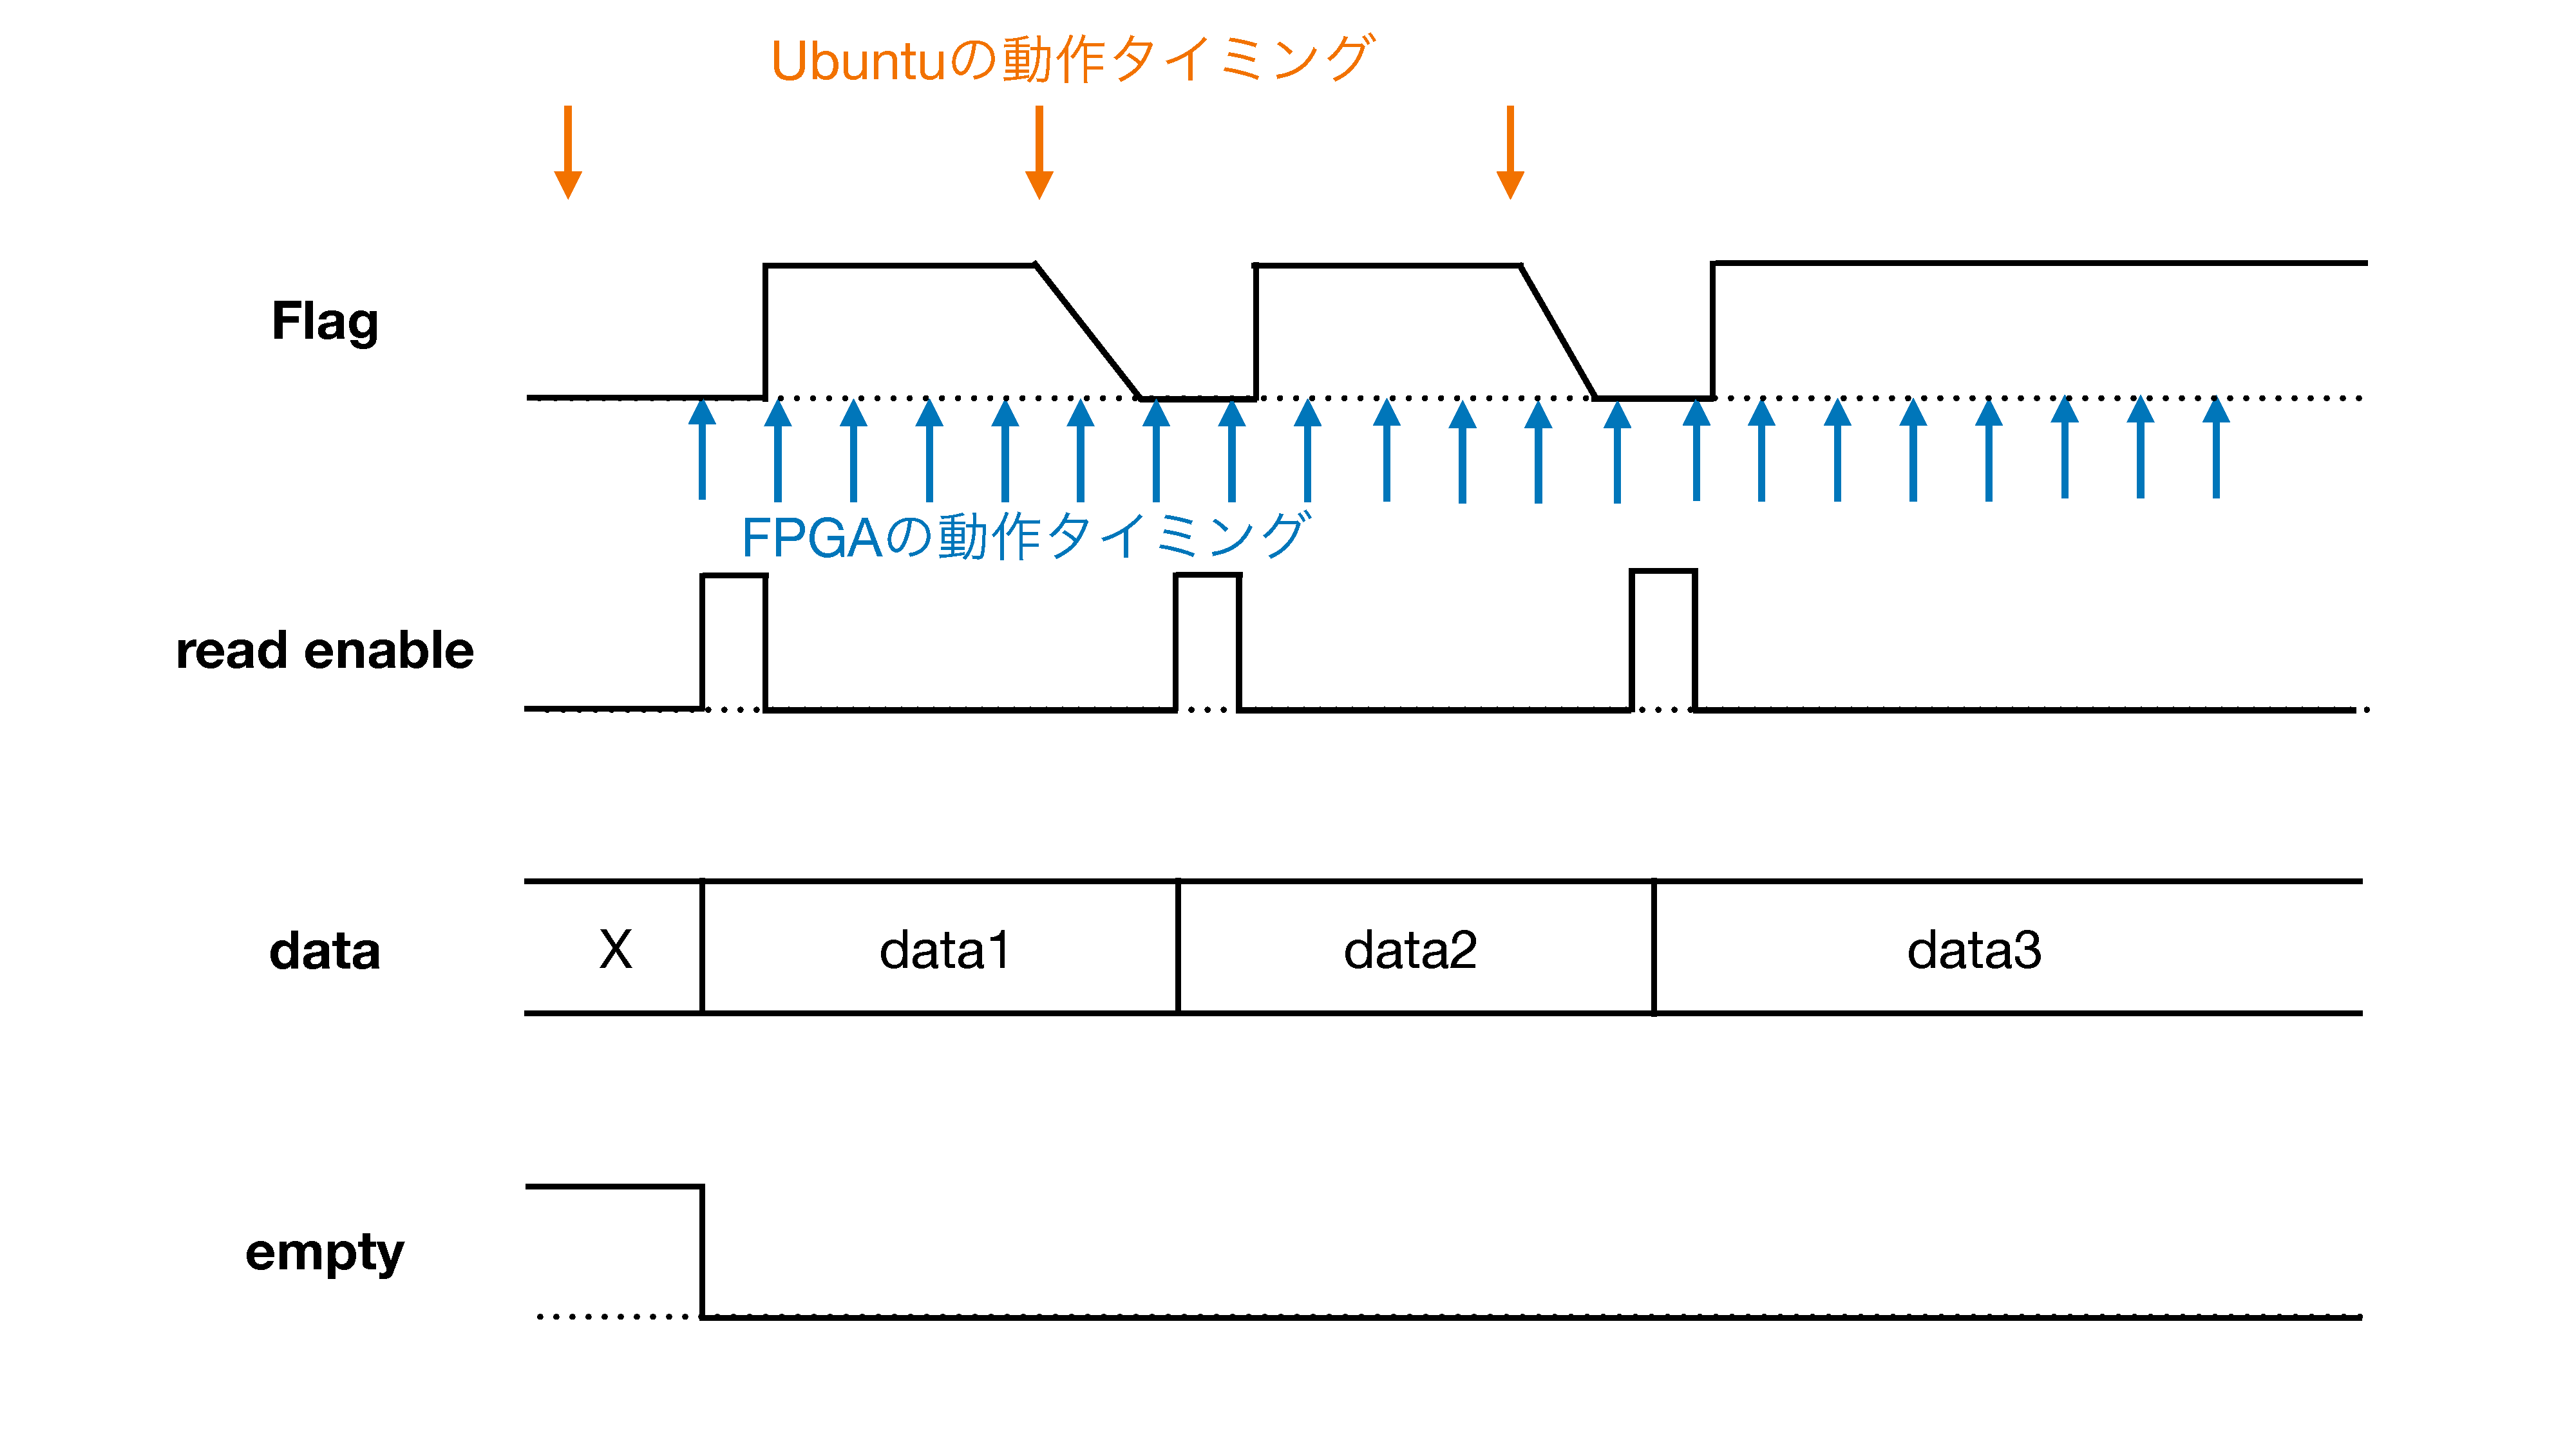
\includegraphics[width=16cm]{fig/QAQC/JATHubarbitation.png}
\caption[調停回路のシークエンス]{調停回路のシークエンス}
\label{JATHubarbitation}
\end{figure}

Ubuntu上のアプリケーションではフラグをモニターし、1になっていたらAXI GPIOレジスタの値を読み出し、その後フラグを1から0にさげる。FPGA上のステートマシンも同様にフラグをモニターし、0になったらFIFOにread enable信号を送信し、その後フラグを0から1に上げる。これによりAXI GPIO レジスタのデータ更新→データ読み出し→データ更新→データ読み出し…の順序が必ず保たれ、もれや重複のない読み出しが実現される。

\subsection{試験に向けた機能実装}
\label{subsec_function}
本節では\ref{sec_QAQCdesign}節で考案した試験を実行するために、JATHub PL部に要請される各機能の実装について述べる。

\subsubsection{コントロール機能}
\label{subsubsec_control}
コントロール機能はLHC 40MHz clockに同期する必要のないスローな制御を担当する。L1AdelayやReadoutBCなどの読み出し回路やTTC制御回路の各パラメーターの設定や、PS board制御のためのレジスタ操作も担当する。この機能によりPS board FPGA内のレジスタ操作やPPASIC、DAC、ADC、Si5395を制御することが可能となる。この機能はZynq PS領域に起動したCPUからPL領域のControl Center内のレジスタ操作により実現する。

\begin{itemize}
\item{\textbf{コントロール回路の全体像}}

FPGA内の各機能の操作はControlCenter内のレジスタ操作により一元的に管理する。図\ref{JATHubccenter}にOSとControlCenterの接続を示す。

\begin{figure} 
\centering
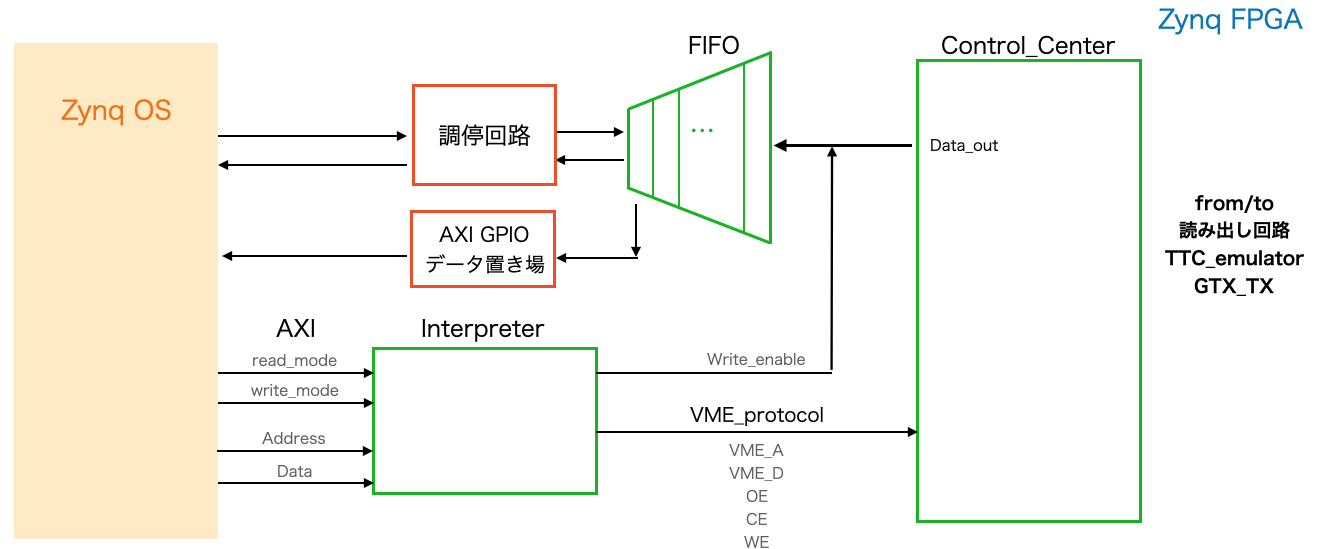
\includegraphics[width=16cm]{fig/QAQC/JATHubccenter.png}
\caption[JATHubコントロール回路]{JATHubコントロール回路。ZynqのOSからPL領域のControlCenter内のレジスタを操作することによりFPGA内の各機能の制御やPS boardへのコントロール信号を制御する。OSからControlCenter内のレジスタ操作はInterpreterが仲介する。ユーザーはアドレスとデータを指定することでVMEプロトコルに従ってレジスタの書き込みを行うことができる。データの読み出しには自作調停回路を利用しており、複数回の読み出しでも安全な設計が実現されている。}
\label{JATHubccenter}
\end{figure}

PS領域からControlCenter内のレジスタ操作はVMEプロトコルを模した自作プロトコルに従って行い、Interpreterが仲介する。ユーザーはPSからアクセスしたいレジスタのアドレスと書き込みたいデータをInterpreterへ伝えることで、Interpreterはプロトコルに従ったバス操作を行い目的の動作を代行する。この実装によりPSからControlCenter内のレジスタへ直接AXIバスを接続する必要がなく、PSからPLに伸びるAXIバスの本数を必要最小限にとどめることができる。また、PS領域とPL領域をつなぐバスが一つしかないため、ControlCenter内の複数のレジスタが同時に書き換えられることを防ぐことができる。ControlCenterからのデータの読み出しには前述の自作調停回路を利用した。
\vskip0.5\baselineskip
\end{itemize}

\subsubsection{\textbf{PS board制御機能}}

PS boardの制御はSLとPS board間で定められた通信フォーマットに従って高速光通信を介して行われる。40 MHzごとに図\ref{JATHubpsbformat}に示すパケットを交換する。SLからPS boardへは各32bitのwordが5word分送信される。QAQC用JATHubにもこのフォーマットに従ったパケットを送受信する機能を実装した。200 MHzで動作するステートマシンにより、40 MHzクロックの立ち上がりと同期したタイミングでWord0が割り当てられ、40 MHzクロックに対して相対的な位相関係が固定されるよう実装されている。PS boardへ送られるソフトリセット信号やテストパルストリガー(Test Pulse Trigger, TPT)信号はControlCenter内のレジスタ操作により設定される。PS board FPGA内のレジスタ操作はword-2、word-3に定義されたAddress,Command,Dataを用いて制御する。Commandにより書き込み/読み出し動作を決め、AddressでPS board内のレジスタアドレスを指定し、書き込みの場合Data bitに値を設定することで書き込みが完了する。
PS board上のDACやPPASICを制御する方法として\ref{subsec_QAQCdesign}節では自立型制御機構を利用するものを述べた。PS board FPGAの状態や各素子のモニターには自立型監視機構を利用する。このシステムではPS board FPGAが自らボード上の素子と通信し、読み出した値を定期的にコントロールマスターに送信する。DACの設定値、ADCの測定値、FGPAの温度、xADCによる供給電圧値などのモニター値は図\ref{PSBdataformat}に示すフォーマットに従い6bitのデータタイプと4bitのデータに分割して送信される。16bitのADCの値は4bitずつ4tickに分割して送信されるため、JATHubでは図\ref{JATHubmonitor}に示すようにデータタイプをもとにモニターデータを再構成し、ControlCenter内のレジスタに格納する。この機能によりPSから任意のタイミングでControlCenterにアクセスすることで常に最新のモニターデータを取得することができる。

QSPIフラッシュメモリーへの書き込み/読み出しはJATHubから直接やSPIプロトコルに従ってビットバンギングすることで行う。ControlCenter内のレジスタを操作することでWord-1で定義されているSCLK、SDIなどを操作する。
\vskip0.5\baselineskip

\begin{figure} 
\centering
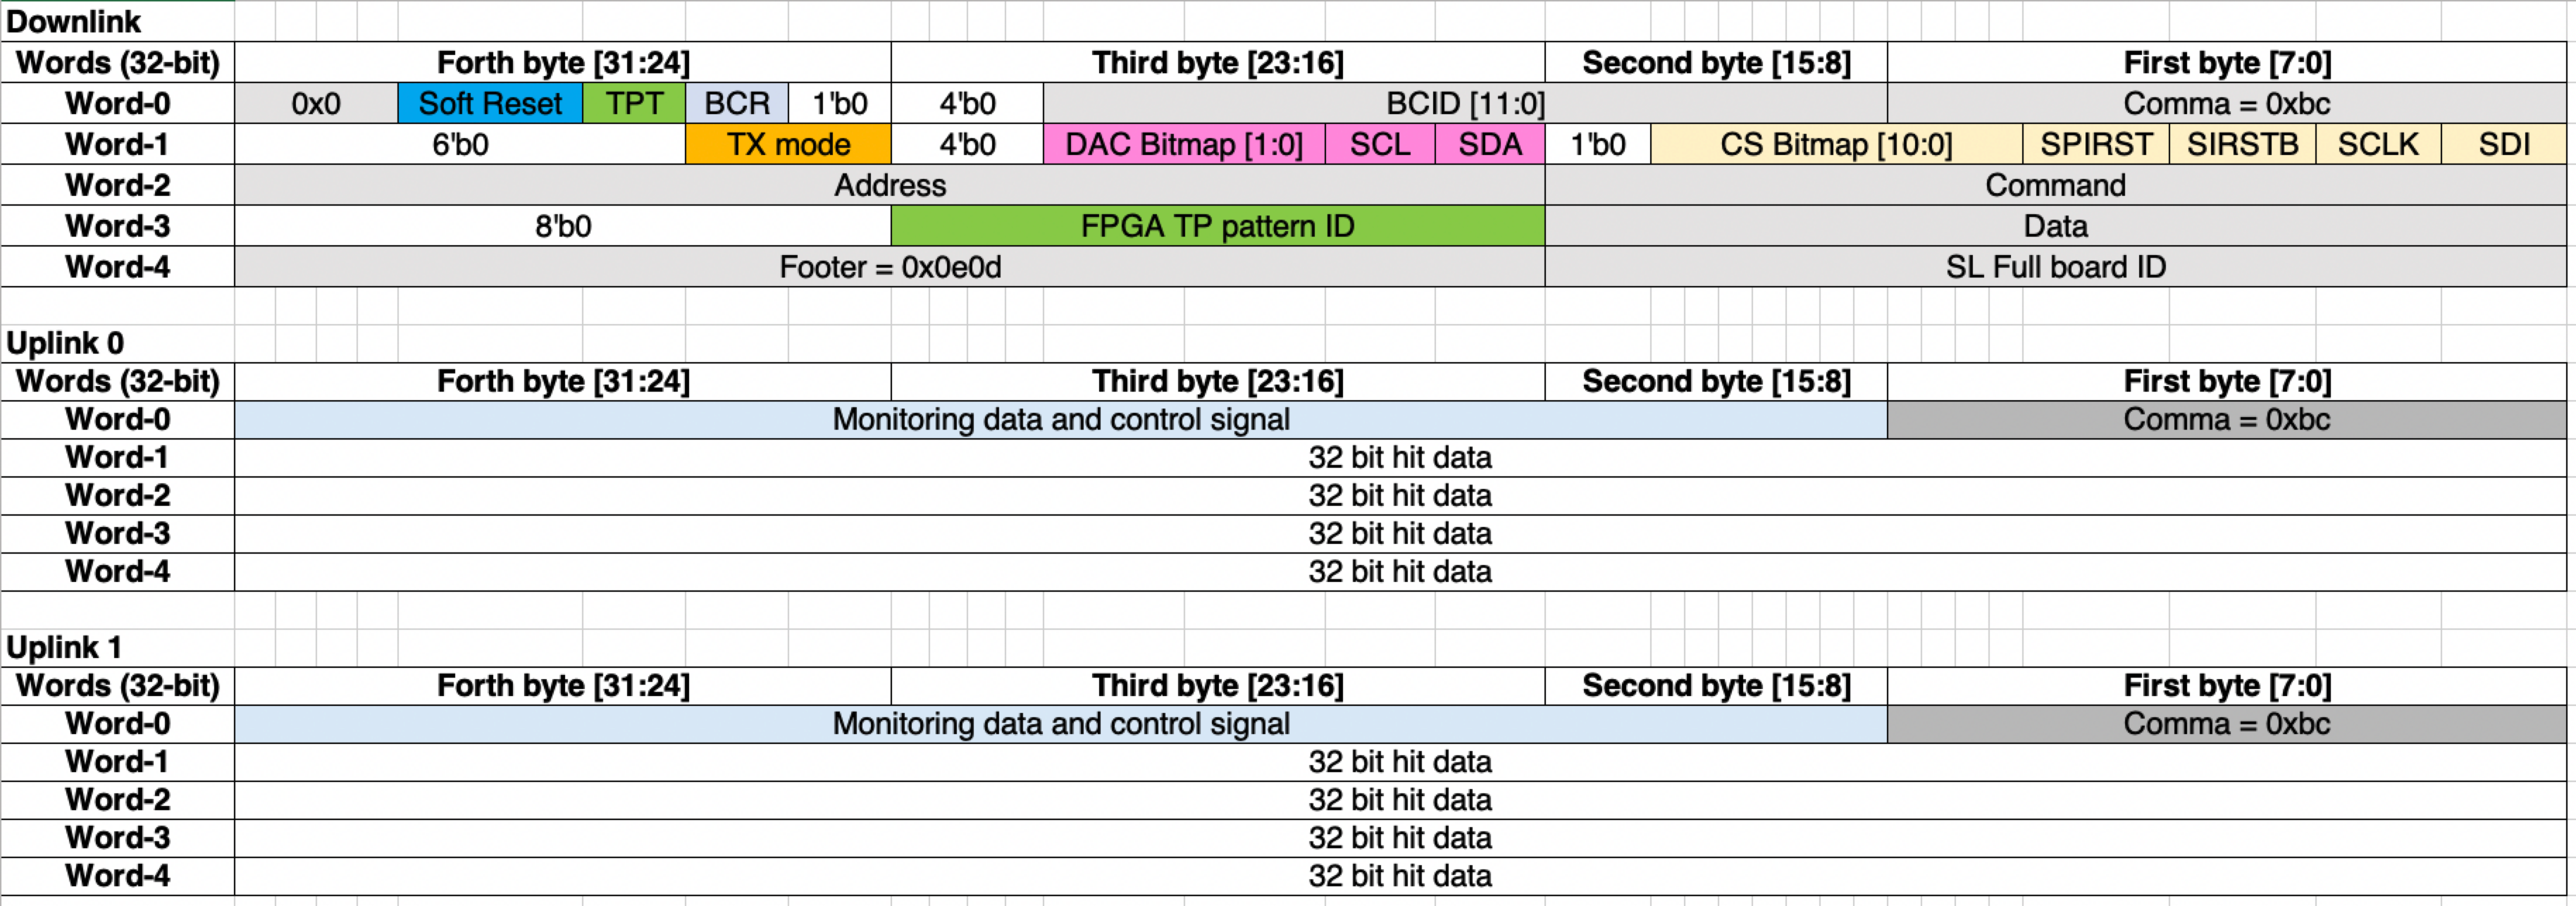
\includegraphics[width=16cm]{fig/QAQC/JATHubpsbformat.png}
\caption[JATHubとPS boardの間で定義された通信フォーマット]{JATHubとPS boardの間で定義された通信フォーマット}
\label{JATHubpsbformat}
\end{figure}

\begin{figure} 
\centering
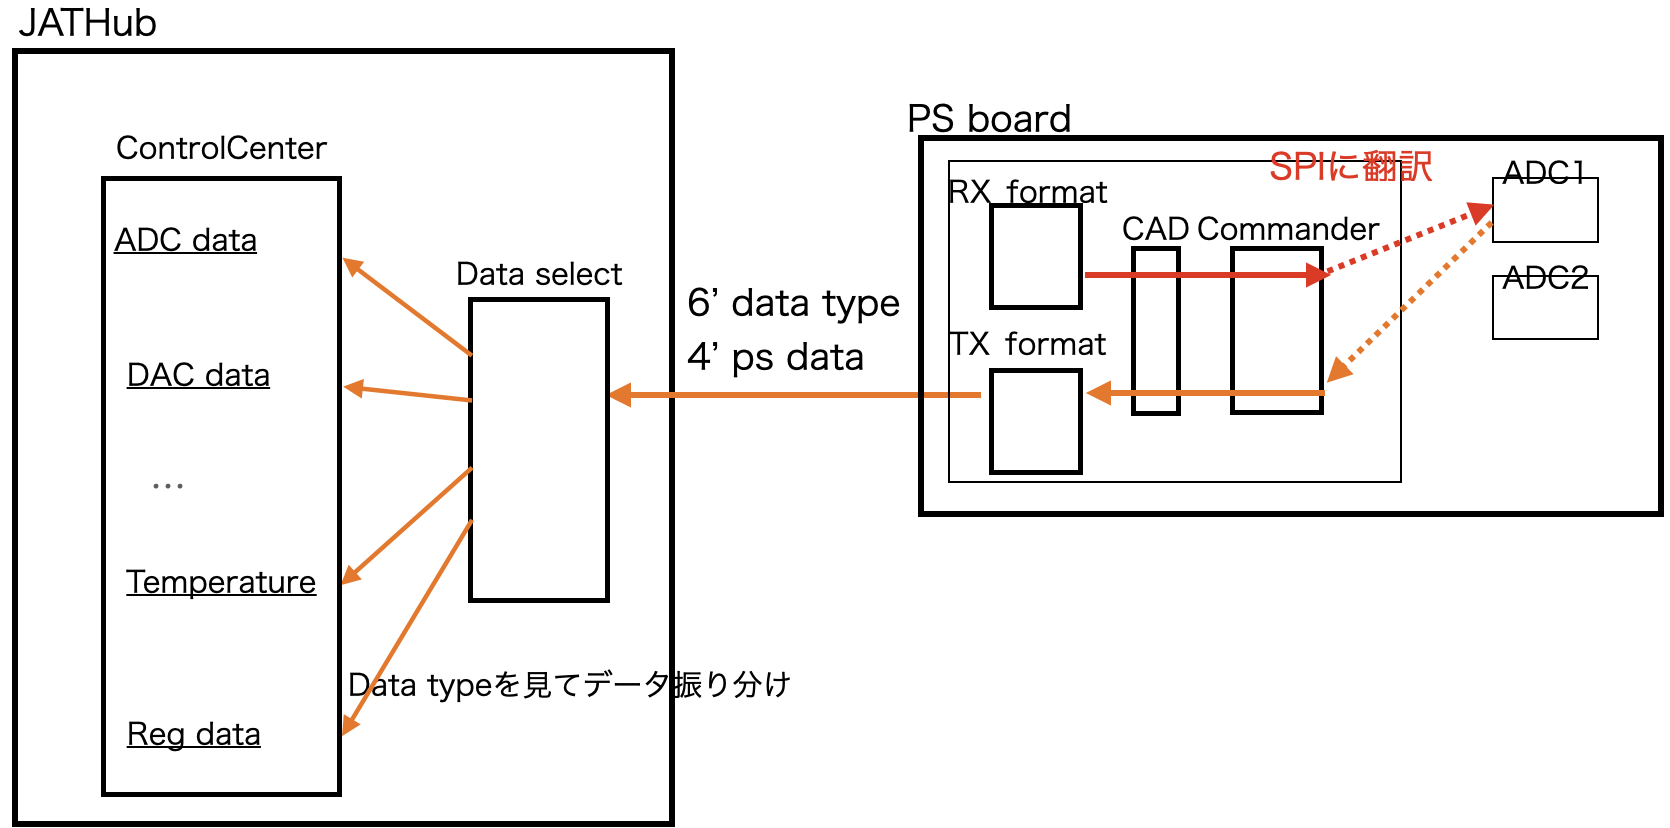
\includegraphics[width=16cm]{fig/QAQC/JATHubmonitor.png}
\caption[JATHub monitor]{JAThubに実装された監視機構。PS boardから送られる制御用データをデコードし、ControlCenter内のレジスタに格納する}
\label{JATHubmonitor}
\end{figure}

\begin{figure} 
\centering
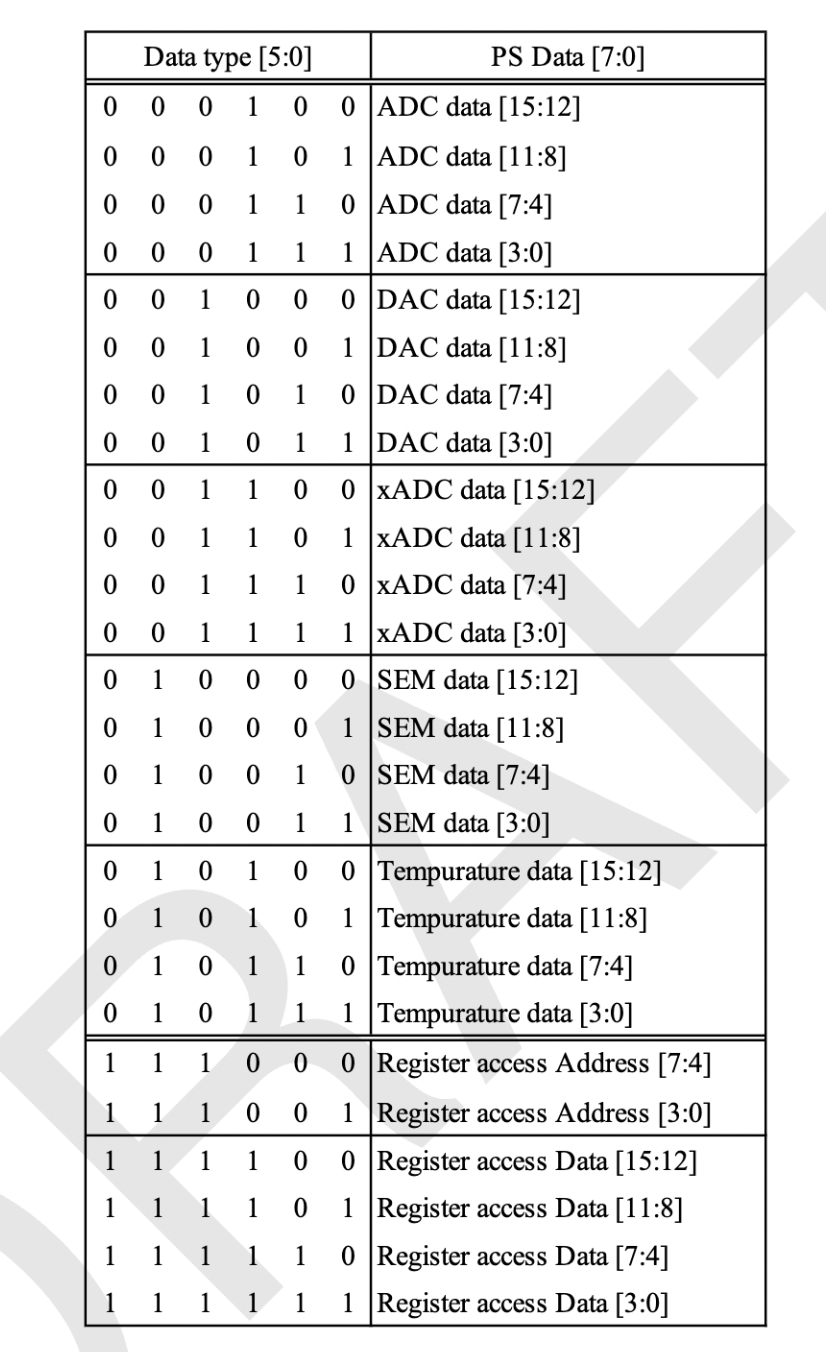
\includegraphics[width=16cm]{fig/QAQC/PSBdataformat.png}
\caption[PS boardから送信されるモニターデータのフォーマット]{PS boardから送信されるモニターデータのフォーマット}
\label{PSBdataformat}
\end{figure}

\subsubsection{ヒットデータ読み出し回路}
\label{subsubsec_DAQ}
読み出し回路の役割はASDテストパルス試験においてPS baordから送信されるヒット信号をJATHub Zynq上のUbuntuから読み出すことである。JATHubは光通信を介してPS boardから25nsごとに256bitのヒットデータを受け取る。40MHzで受け取るデータとそのデータに割り当てられたタイミング情報(BCID、L1ID)をFPGA上でバッファーしておき、TPTと同期してL1Aを発行することで、テストパルスデータを選択的に取り出しFIFOメモリーにダンプする。FIFOメモリーに貯蓄されたデータはCPUの動作する任意のタイミングにおいてCPUから読み出せるよう調停回路を介して読み出させる。
この実装の全体像を図\ref{JATHubreadout}に示す。

\begin{figure} 
\centering
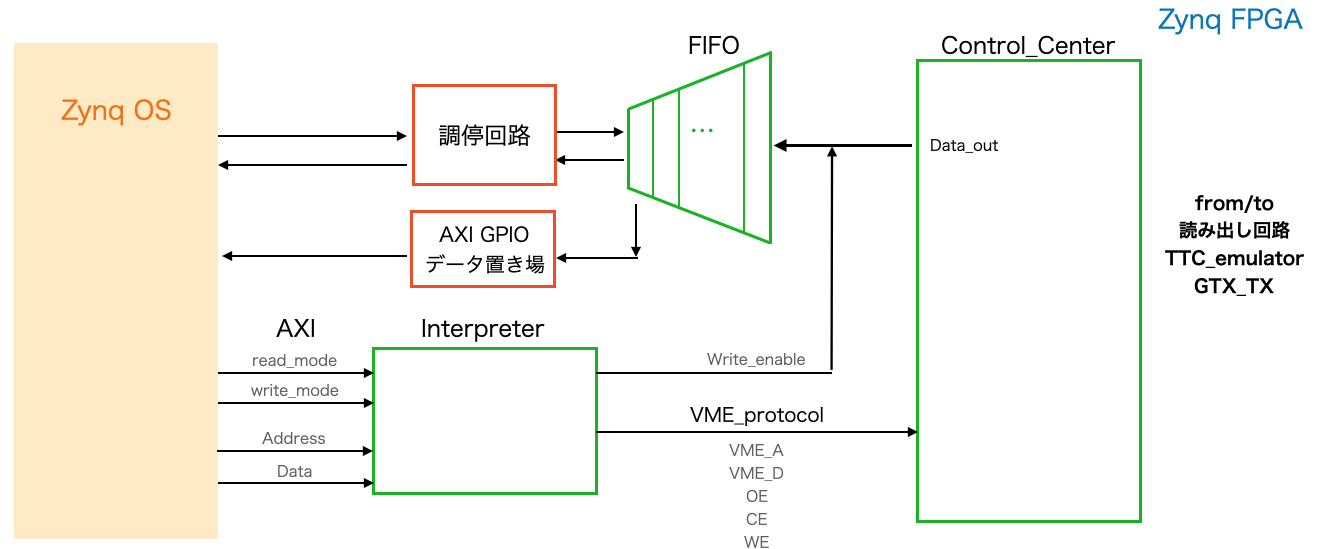
\includegraphics[width=16cm]{fig/QAQC/JAThubreadout.png}
\caption[読み出し回路の全体像]{読み出し回路の全体像}
\label{fig_CTA}
\end{figure}

\begin{itemize}
    \item \textbf{TTC emulator} \par
    ASDテストパルス試験ではJATHub、PS board、ASDが共通のクロックを共有し、同期して動作する必要がある。本システムではJATHub上の水晶発振器で生成された200 MHzクロックを分周してLHCバンチ交差クロックを模した40 MHzクロックを作成し、それを基準クロックとして利用する。Phase-2 TDAQシステムにおいてFELIXが発行する、Bunch Crossing Reset(BCR)信号やEvent Counter Reset(ECR)などのTrigger Timing Control(TTC)信号もJATHub内で生成しPS boardへと分配する必要がある。この役割を果たすのがTTC emulatorである。ここで発行されたTTC信号は通信フォーマットのWord-0に埋め込まれ、光通信を介してPS boardへと伝えられる。TTC emulatorはTPT信号とLevel 1 Accept(L1A)信号を同期して管理している。TGC L1 TDAQは固定レイテンシーでのDAQシステムになっている。TPTを発行してから、PS boardよりテストデータが返ってくるまでのレイテンシーをあらかじめ計測して一度L1A depthを調整すれば、以降は固定レイテンシーでのデータ読み出しを実現することができる。いかにTTC emulatorを構成する各モジュールの役割を説明する。
    \vskip0.5\baselineskip

    \begin{itemize}
        \item {TTC generator :} 40MHz LHC clockで動作するカウンター。reset信号でカウンターをリセットし、1クロックチック毎にカウンターの値を1ずつつインクリメントする。カウンターの値が3564に達したタイミングでBCR信号を発行する。デフォルトの設定ではTPT、L1AもBCRに合わせて3564 BCに一回発行しているが、任意のタイミングでTPT、L1Aを発行することも可能である。TPT lengthを変更することですることでTPTを複数BCに渡って出力することも可能である。
        \vskip0.5\baselineskip

        \item{TTC Delay :}1bit幅、深さ4096のBRAMで実装したdelay回路。L1A、BCR、TPTに任意の遅延をかけることができる。L1A Delayを調整することでTPTからL1Aを発行するまでのレイテンシーを変更することができる。
        \vskip0.5\baselineskip

        \item{ID counter :}BCR、ECR、L1Aを受けてBCID、ECID、L1IDを数え上げるカウンター。ここで発行されたBCIDやL1IDはUbuntuからの読み出しフォーマットに組み込まれて出力される。読み出したデータのL1IDの連続性やBCIDを確認することでデータの欠損や重複を検出することができる。
        \vskip0.5\baselineskip
        
        \item{FPGAテストパルス発行機能 :}PS boardの持つFPGAテストパルスを発行するためのモジュール。FPGAテストパルスはPS board内のBRAMに保存される。BRAMのaddressを指定した状態で、TPTを発行するとBRAMから256bitのヒットビットマップが取り出され、ASDからのヒット信号に代替してJATHubにデータを送る。
        \vskip0.5\baselineskip
    \end{itemize}

    \item \textbf{L1 Buffer} \par
    L1BufferはPS boardから受信した256bitのヒットビットマップとECRID,L1ID,BCID,SLIDなどのタイミング情報を合わせた432bitのデータを一時格納するためのリングバッファーである。ttc emulatorからL1Aが出されたイベントは後段のDerandomizerに転送され、それ以外のデータはここで捨てられる。40MHのLHCバンチ交差クロックに同期して到着する入力ビットマップは、書き込みポインタが示すアドレスに格納される。書き込み用ポインタと読み出し用ポインタはLHCバンチクロックに同期して1ずつインクリメントする。書き込み用ポインタがBRAMの最後尾まで達した場合、次のクロックチックで再び先頭に戻る。L1 Depthによって書き込み用ポインタと読み出し用ポインタのアドレスの差を設定することができ、Bufferの深さを任意の値に設定することができる。L1Aが発行されてから何BC分のデータを読み出すかをReadout BC inによって設定することができる。defaltでは3に設定されており、一回のL1Aに対してprevious,current,nextの3イベント分を読み出すことができる。ReadoutBCで設定されたBC分のデータを読み出している途中に再度L1A信号を受信すると、読みだしエラーを出力される。読み出しエラーが生じたL1IDをControlCenter内のレジスターに格納し、ユーザーが確認できるようになっている。
    \vskip0.5\baselineskip

    \item \textbf{Derandomizer} \par
    Derandomizerは後段で行われるUbuntuからの読み出し処理待ちBufferであり、432bitの入力データをUbuntuからの読み出しに適した32bitずつ出力する。DeranomizerはFIFOを2つ直列に並べることで実装している。FIFO1は432bitの入力ビットマップに16bitのheader、64bitの不要データを付け加えた512bitの入力を64bitずつ出力する。FIFO2は64bitの入力を受けて32bitずつ出力する。データ幅の縮小にはFIFO IPの持つ入力データをスライスして出力する機能を利用している。スライス幅は2、4、8が用意されている。Derandomizerからの出力はUbuntuのInt型と整合性のある32bitが好ましく、32bitの出力を得るために二つのFIFOを直列に繋いでいる。また32bitの16倍である512bit の入力に合わせるために64bitの不要データを付け加えている。64bitの不要データはFIFO1からFIFO2の間で捨てられるような設計になっていてUbunutuからの読み出しには関係しない。FIFOは入力されたデータを順番に出力する特性を持ったメモリーである。書き込みと読み出しを非同期に行うことができ、一般にクロックドメインをまたぐデータの送受信に利用される。本システムでは固定レイテンシーで動くFPGA内の読み出し回路とPS領域からのデータ読み出しをつなぐ目的で使用する。Derandomizerへの書き込み動作は40 MHzクロックの固定レートで動作し、それ以降の読み出しは回路は240MHzで動作させる。Derandomizerへのデータ書き込みレートがUbunruからの読み出しレートを上回る場合にはDerandomizerのoccupancyは増大していく。その状態が続くとバッファーのオーバーフローが発生しデータが欠損する。バッファーオバーフローが生じた際への対応はのちに紹介する。
    \vskip0.5\baselineskip

    \item \textbf{イベントビルダー} \par
    イベントビルダーはDeradomizerに格納されている32bit幅のワードを240MHzのクロックチック毎に1ワードずつ順番に読み出し、図\ref{JATHubhitformat}に示す読み出しフォーマットに整形する。PS boardから受信した256 bit x 3 BC分のデータに加えて、TTC emulator から発行されたTTC信号(ECRID、L1ID、BCID)、PSBから発行されたTTC信号も同時に読み出す。JATHub内で割り当てら得たBCIDとPS boardから返ってきたのBCIDの差を確認することで、固定レイテンシーでのDAQが実現できていることを確かめることができる。
    \vskip0.5\baselineskip

    \item \textbf{読み出し回路の性能} \par
    実装した読み出し回路の性能として、データ読み出しレートを概算しておくことは試験設計において重要である。ASDテストパルス試験におけるTPT発行レートなどは読み出しレートに制限される。Ubuntu上で実行時間を測定するためのappを走らせ、FIFOに格納された1000イベント分のパケットを読み出すのにかかる時間を測定した。図\ref{JATHubreadspeed}にその結果を示す。
    横軸に読み出したパケット数、縦軸に経過時間(s)をとる。得られた測定結果を線形フィットしてその傾きから1パケット読み出すのにかかる時間を測定したところ$85 us/packet$となった。

    \vskip0.5\baselineskip
    \begin{figure} 
    \centering
    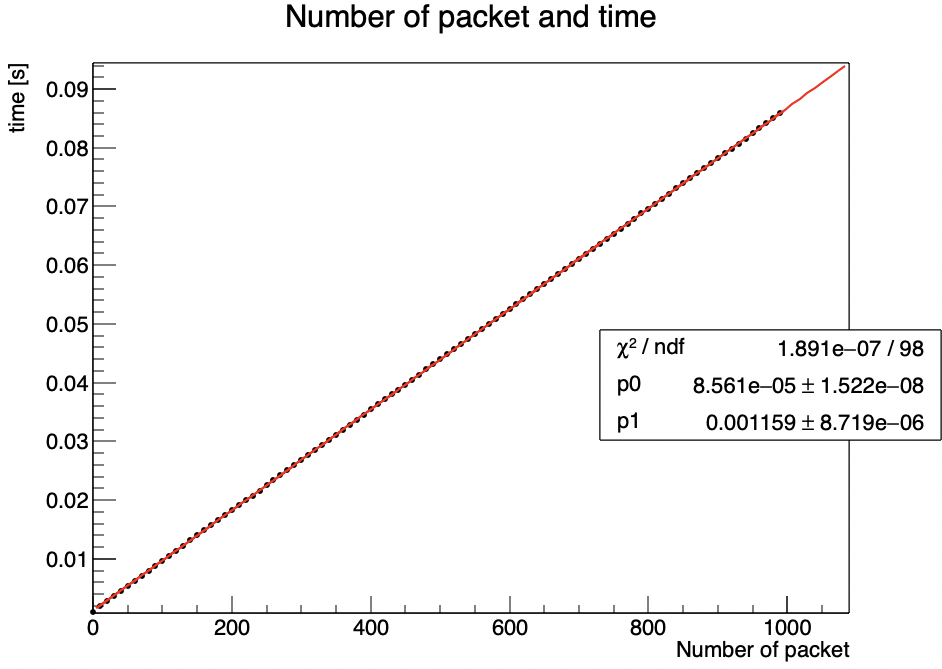
\includegraphics[width=16cm]{fig/QAQC/JTAHubreadspeed.png}
    \caption[PSからのヒットデータ読み出し速度の測定]{PSからのヒットデータ読み出し速度の測定}
    \label{JTAHubreadspeed}
    \end{figure}

    \item \textbf{バッファーオーバーフローへの対応} \par
    万が一バッファーオーバーフローが生じた時においても、イベントパケットが崩れることのないようにバックプレッシャー機能を実装した。Derandomizerに保存されたデータがあらかじめ設定した容量閾値(4000/4096)を超えるとL1 Bufferへalmost full信号が送らる。almost full信号を受け取ったL1Bufferは処理中のイベントのデータを出力を完遂させたのち(Previousの出力中にalmost full信号が来た場合、current,nextデータまで出力を終えたのち)、L1Aを受け付けなくなる。オーバーフローが起きた場合においてもTTC emulatorからのL1Aの発行は止まらないが、L1 BufferからDerandomizerの間でデータが捨てられる。ASDテストパルス試験ではUbuntuから読み出したイベント数に対してヒットデータが入っていた割合を計測するため、L1 Bufferで捨てられたイベントについては試験結果に影響しない。
    \vskip0.5\baselineskip

    \begin{figure} 
    \centering
    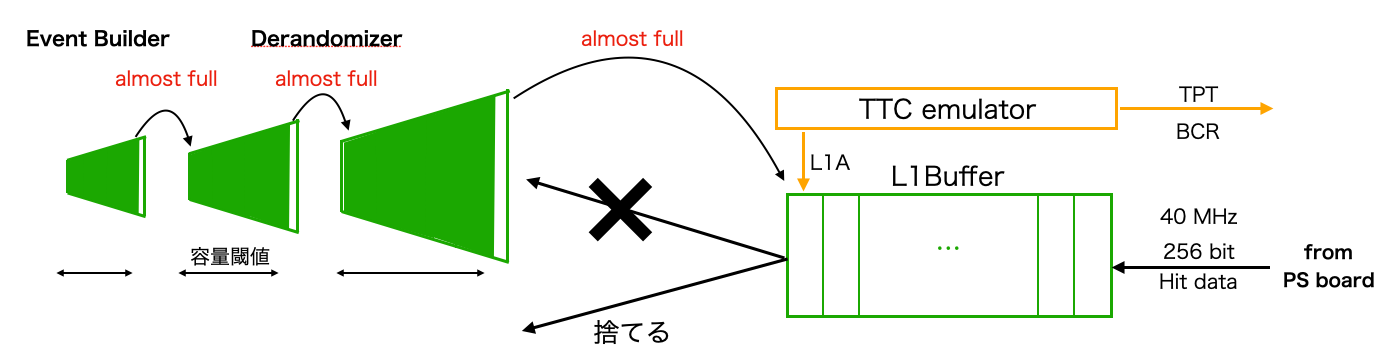
\includegraphics[width=16cm]{fig/QAQC/JATHubbackpressure.png}
    \caption[リードアウト回路におけるバックプレッシャー機能]{リードアウト回路におけるバックプレッシャー機能}
    \label{JATHubbackpressure}
    \end{figure}

\end{itemize}


\subsubsection{JTAG/Recovery/Clock位相測定機能}
\label{subsubsec_jtagrecovery}
Cat 6ケーブル経由でのJTAG通信によるファームウェア書き込み、Recovery線によるリカバリー機能、PS boardから送信されたクロックの位相測定機能は先行研究で開発されており、それらの機能を本システムにも統合した。
\begin{itemize}
    \item \textbf{SVFプレイヤー} \par
    PS部に起動したUbuntuでSVFファイルを読み込み、JTAG4線をドライブする機能。
    \vskip0.5\baselineskip

    \item \textbf{Recovery機能} \par
    PS board FPGAのレジスタ操作によりPS boardからRcvB線を経由してリカバリーリクエスト信号を出させる。リカバリーリクエストを受け取ったJATHubからPROGBをアサートし、PS board FPGAをリセットする。
    \vskip0.5\baselineskip
    
    \item \textbf{クロック位相測定機能} \par
    MON線経由で送られる40 MHzクロックの位相をJAThub内の水晶発振器から生成した40 MHzクロックを参照クロックにして測定する。システムの概念図を図\ref{JATHubclockmeasure}\cite{mt_atanaka}に示す。Vivadoで提供されるClocking WizardというIPを用いて参照クロックを1/56 ns刻みで位相をシフトすることができる。この機能を用いて参照クロックをシフトさせながら、参照クロックの立ち上がりでPS boardからのクロックをサンプリングすることでクロックの位相を測定する。
    \vskip0.5\baselineskip

    \begin{figure} 
    \centering
    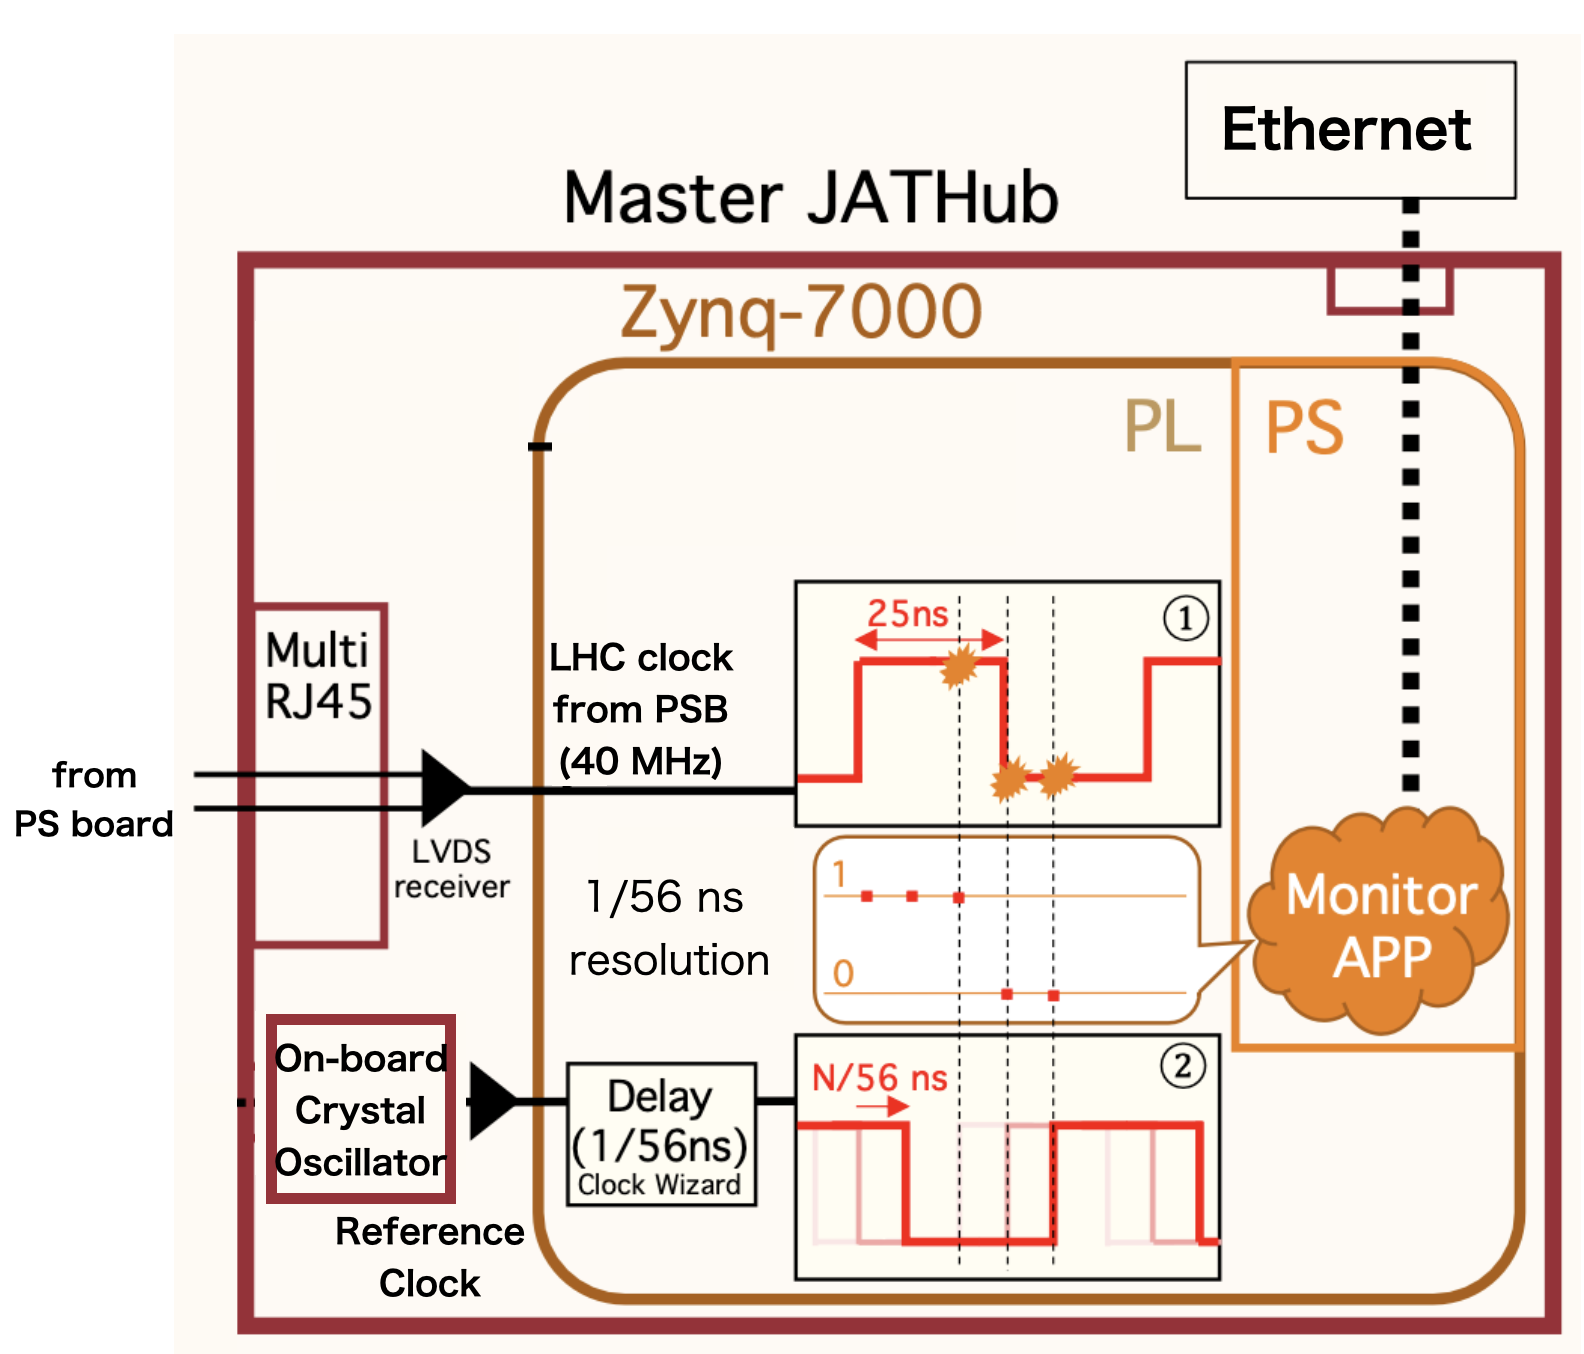
\includegraphics[width=16cm]{fig/QAQC/JATHubclockmasurement.png}
    \caption[JATHubによるクロック位相測定の概念図]{JATHubによるクロック位相測定の概念図}
    \label{JATHubclockmeasure}
    \end{figure}

    \end{itemize}

\section{PS board QAQC試験デモンストレーション}
\label{sec_PSboardQAQCdemo}

\subsection{試験環境}
\label{subsec_testenv}
東京大学に設置したテストベンチを利用して\ref{4-2}節で開発したQAQC用JATHubの動作検証及びQAQC試験のデモンストレーションを行なった。

セットアップを図\ref{QAQCsetup}に示す。QAQC用のJATHubはVMEクレートに設置しバックプレーンのJ3コネクターを経由して電源を入れる。PS boardには3.3V デジタル用電源、3.0Vデジタル用電源、-3.0Vようアナログ電源を用意しデスクトップで給電した。JATHubとPS boardは2リンクの光リンクと2本のCat 6ケーブルで接続する。1台のPS boardには8台のASDを接続する。試験を行なった2023年11月時点ではRJ45とPHYチップを搭載したJATHub量産機は生産途中であったため、uart経由でZynq上に起動したUbuntuを操作する。

3-1節では本セットアップにおいてPPASICのパラメーターを決定するために行なった試験について述べる。
3-2 節ではQAQC試験を通して行なった際の所要時間を示す。
3-3節では本試験で明らかになった時間削減の必要性とそのための試験並列化のアイデアおよび実装について述べる。
最後に3-4節では本QAQC用JATHubの汎用性を活かしたその他の実験でのシステム使用例について言及する。
\vskip\baselineskip

\subsection{テストベンチにおける機能検証試験および試験パラメーターの決定}
QAQC試験では量産個体に対する試験に先んじて、PPASICの遅延、DACの閾値電圧、L1A depthパラメーターを設定しておく必要がある。

\subsubsection{PPASIC遅延パラメーター}
PPASICの遅延パラメーターは使用するシグナルケーブルの長さに依存するパラメーターである。ASDからのテストパルス信号の立ち上がりがPPASICにおけるLHCバンチ交差クロックの立ち上がりと極めて近い場合、PPASICでのBCIDが多少のフラクチュエーションによって2つのBCにまたがる可能性がある。これを防ぐため、両者の立ち上がりが十分離れるようパラメーターを設定する。そのために行なったディレイスキャンの結果を図\ref{QAQCdelayscan}に示す。陽子バンチ識別回路の有効ゲートを25 ns、可変遅延回路の刻みはばを1.19 nsに設定した。PP ASICの遅延パラメーターを変えていきながらテストパルス試験を行い、測定されたefficiencyをPrevious、Current、NEXTそれぞれについて記録した。遅延パラメーターを変更するごとにテストパルスがPreviou, Curretn, NEXT BCとBCIDされていることがわかる。この試験によりQAQC試験で利用するパラメーターを 20 nsと決定した。
\vskip0.5\baselineskip

\begin{figure} 
\centering
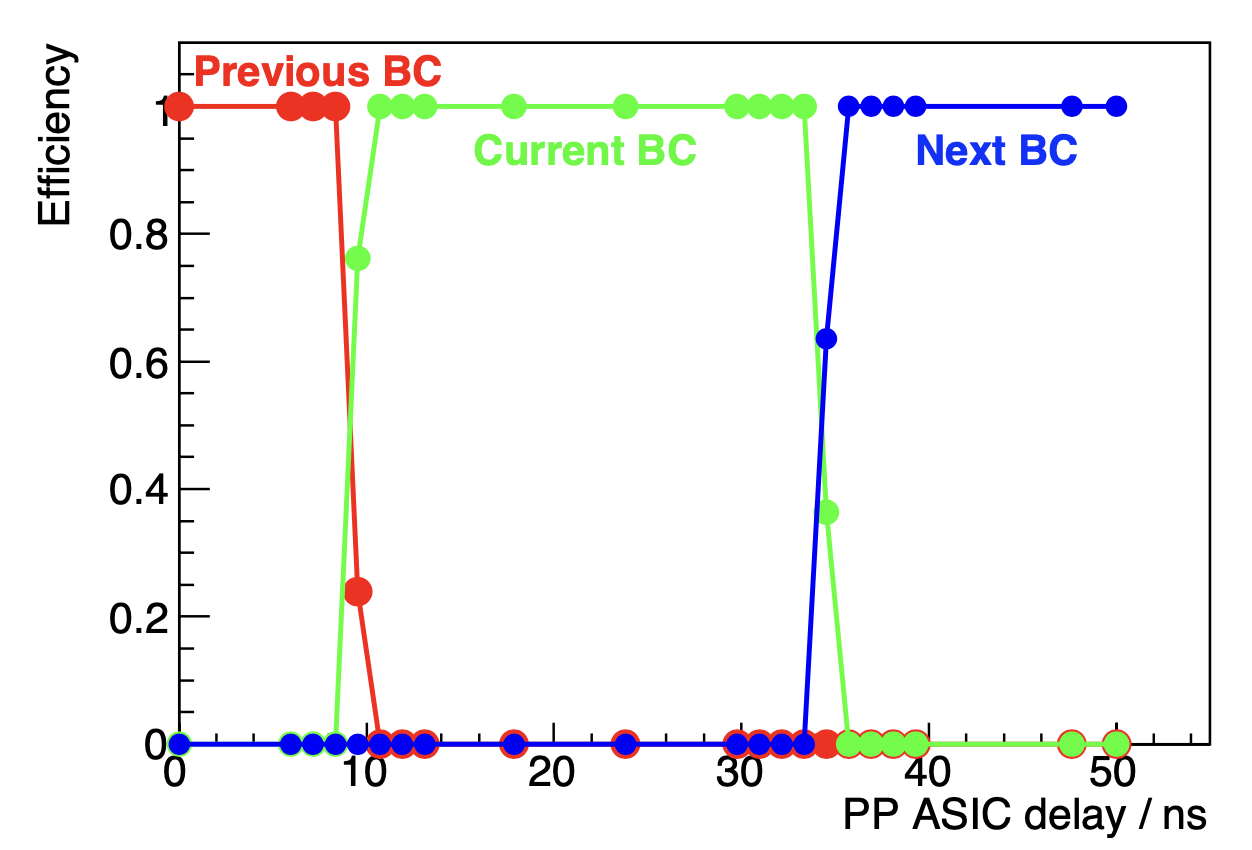
\includegraphics[width=16cm]{fig/QAQC/QAQCdelayscan.png}
\caption[ディレイカーブ]{テストベンチで測定したdelay curve}
\label{QAQCdelayscan}
\end{figure}

\subsubsection{L1Adepth}
L1AdepthはL1Bufferの深さを決めるパラメーターであり、TTC emulatorでTPTを発行してからPS board からヒットデータが返ってくるまでのレイテンシーに合わせて調整する必要がある。主にPS boardからJATHubの間の光ケーブルの長さに依存するパラメーターである。本セットアップでは上の試験と合わせて設定を行なっており、0x87に設定した。
\vskip0.5\baselineskip

\subsubsection{ノイズスキャン}
DACの閾値電圧は使用するASDのノイズの大きさに依存して変えるべきパラメーターである。ASDには元から数十mVの固有のノイズが乗っていることが知られており、それよりも閾値電圧を低く設定してしまうと、ノイズもヒット信号として処理してしまい期待した試験ができない。閾値電圧はノイズの値よりも高く、かつテストパルスの値より十分低く設定すべきである。そこでDACの閾値電圧を変えながらテストパルスを測定するノイズスキャンを行なった。その結果を図\ref{QAQCnoisescan}に示す。
閾値電圧を変えていき、0 ~ 50 mVになるとノイズによるヒットレートが上昇し、その後再びノイズは消えていく様子がみてとれる。この結果から本セットアップでのDAC閾値は+-それぞれ+70 mV、-40 mVと設定した。
これらのパラメーターをもとにASDテストパルス試験を行なった結果を図\ref{QAQCresult}示す。全てのチャンネルでCurrentのefficiencyのみ1となっており、PS board上の各種パラメーターの設定が期待通り行えていること、また固定レイテンシーでの読み出しが実現できていることを確かめることができた。
\vskip0.5\baselineskip

\begin{figure} 
\centering
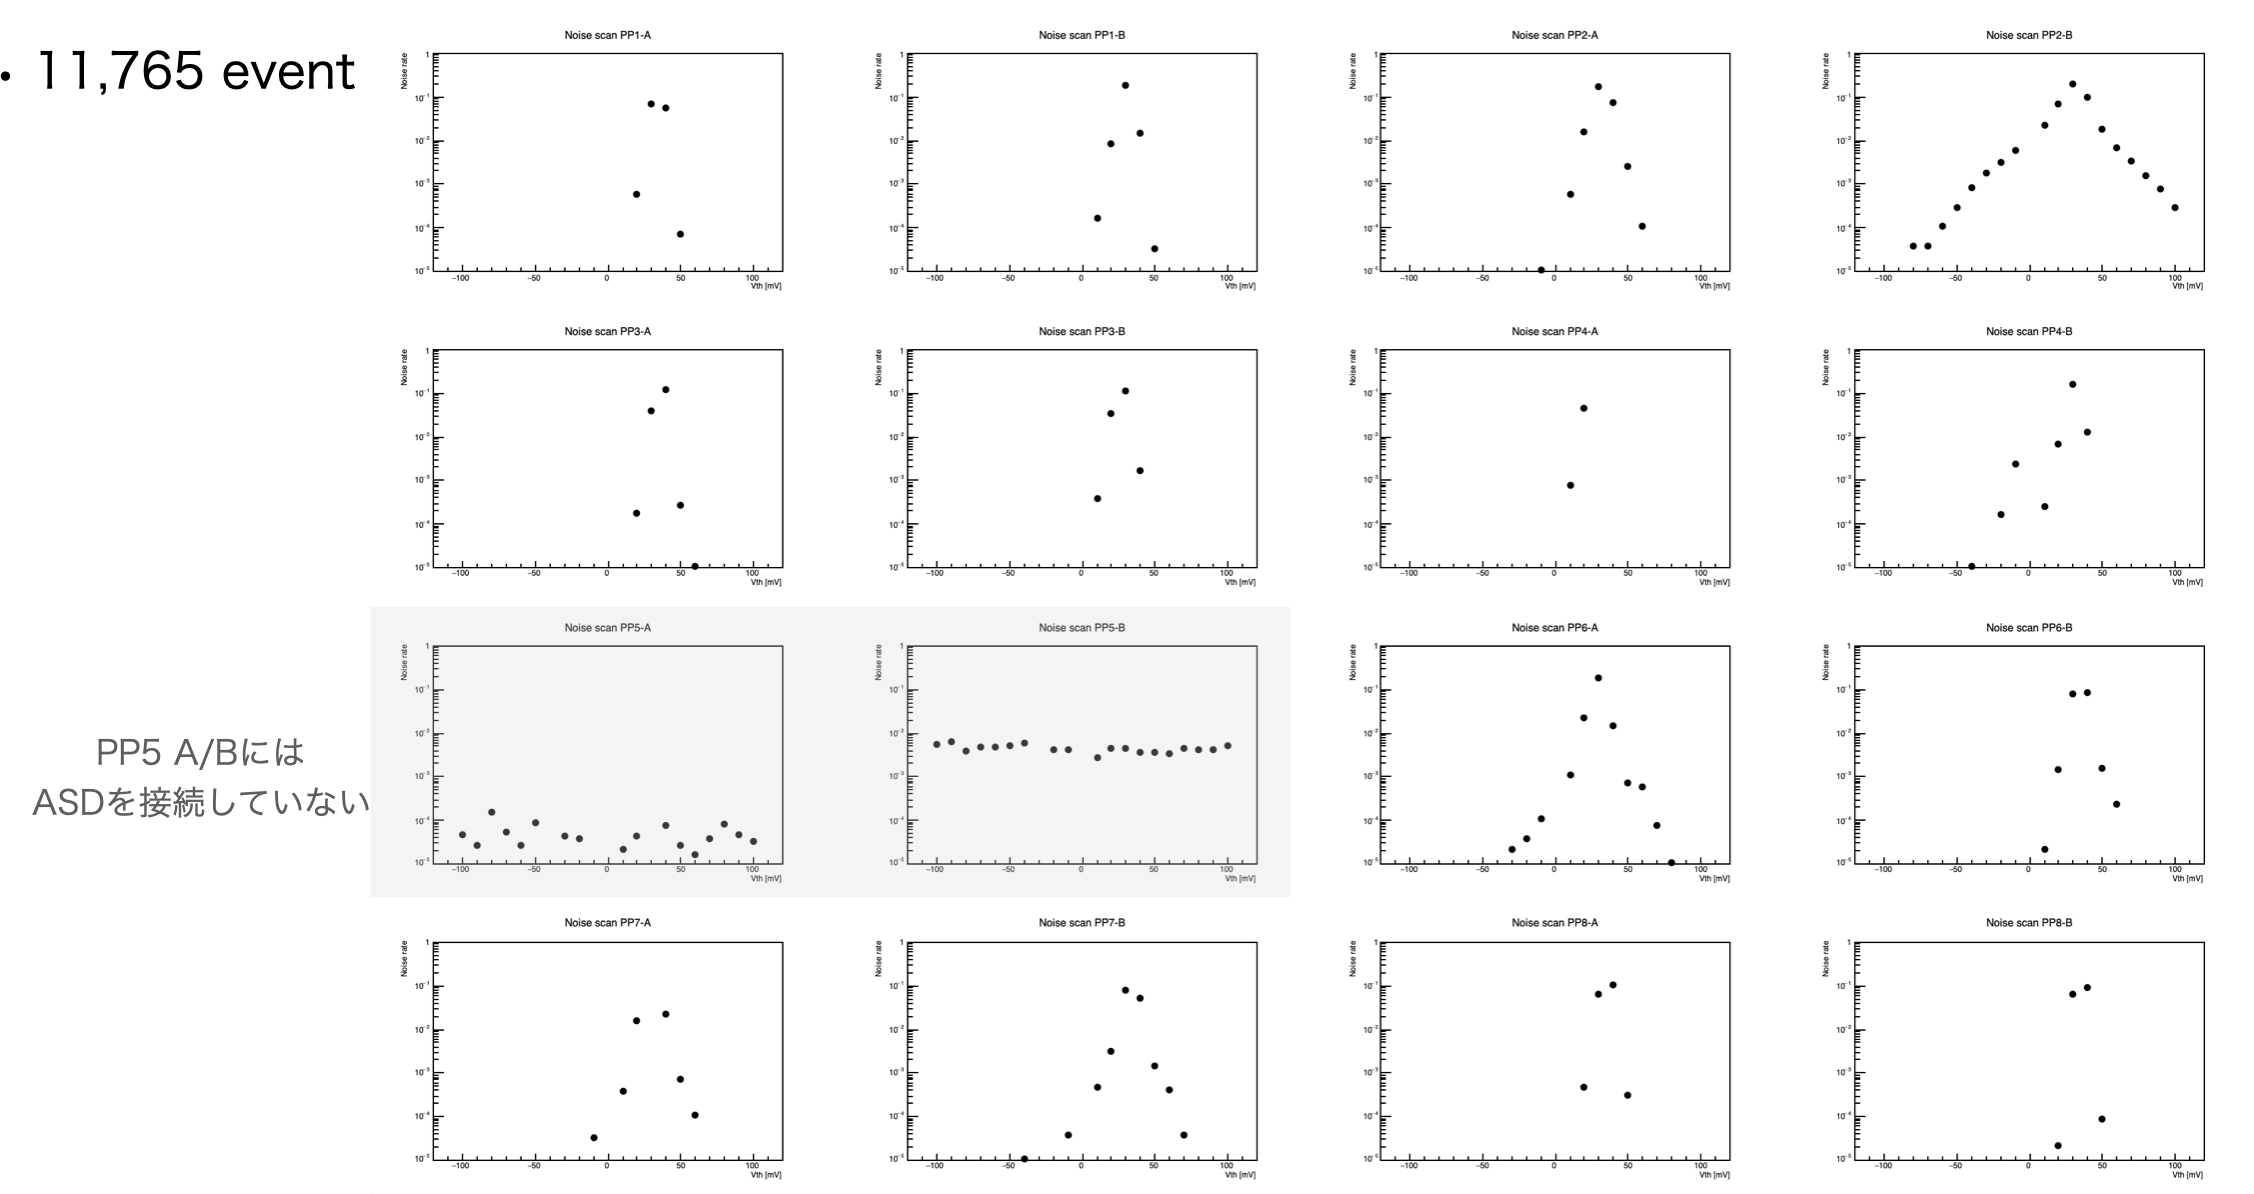
\includegraphics[width=16cm]{fig/QAQC/QAQCnoisescan.png}
\caption[ノイズスキャン]{ノイズスキャンの結果}
\label{QAQCnoisescan}
\end{figure}

\begin{figure} 
\centering
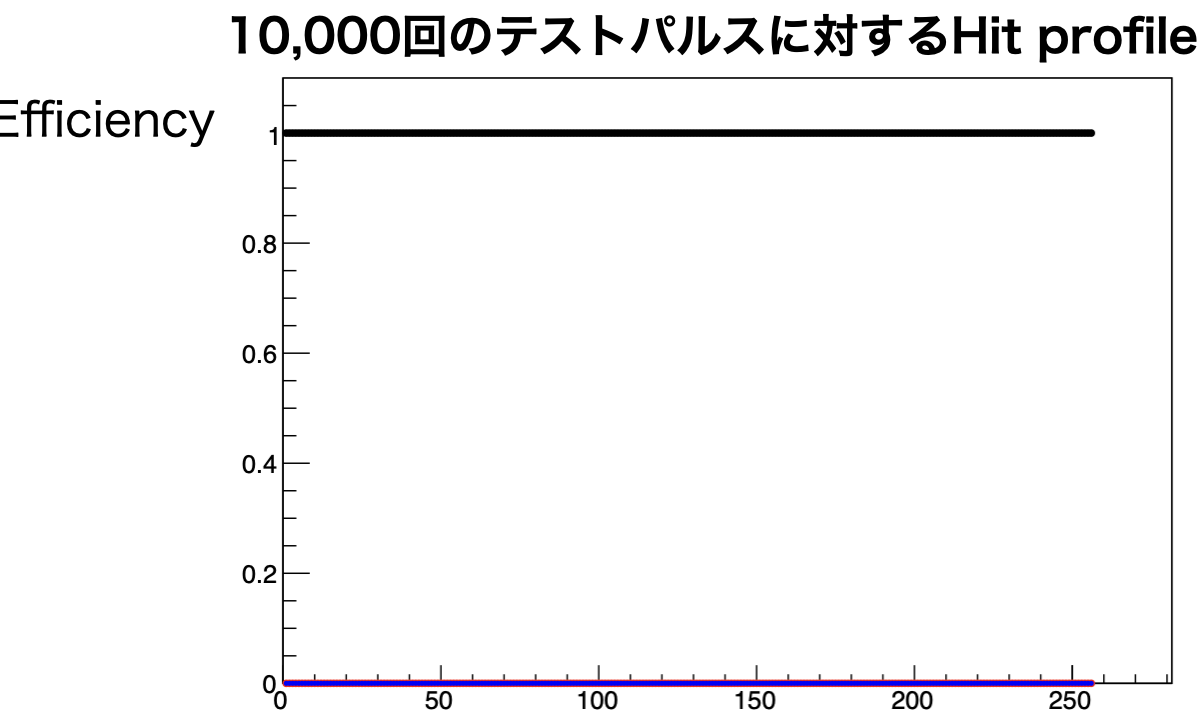
\includegraphics[width=16cm]{fig/QAQC/QAQCresult.png}
\caption[ASDテストパルスの結果]{ASDテストパルス試験の結果}
\label{QAQCresult}
\end{figure}

またその他の試験でも期待通りの結果が得られ、QAQC用JATHubシステムの実装が完了したことを確認した。以下にその所要時間を示す。

\begin{table}[]
    \begin{tabular}{lllll}
    SVFプレイヤーによるQSPIファームウェア書き込み    & 30 min &  &  &  \\
    QSPIパラメーター書き込みおよび読み出し         & 2 min  &  &  &  \\
    リカバリー試験                       & 1 s    &  &  &  \\
    電圧値のモニタリング(ADC、XADC) & 2 s    &  &  &  \\
    Clock位相測定                     & 30 s   &  &  &  \\
    ASDテストパルス試験                   & 10 s   &  &  & 
    \end{tabular}
\end{table}

\subsubsection{試験並列化のためのシステムアップグレード}
\label{subsubsec_parallel}
1枚のPS boardを試験するのに50分以上かかることが明らかになった。この試験を1500枚のPS boardに対して行うのは現実的でない。そのためJATHub1台とPS baord 1台からなる検査セットを20セット並列に試験を行うためのシステムを開発した。
試験並列化のための試験セットアップを図\ref{QAQCpararell}に示す。20の各検査セットは1台のJATHub masterのslaveとして動作する。ユーザーはmasterのJATHubみを操作して、各スレーブJATHubに対して試験開始の命令を出したり、試験状況をモニターしたりする。JATHub masterからJATHub slaveへのコミュニケーションはVMEマスターとしてTAMボードを利用する。JATHubからTAMへは8Gbpsの光通信を行い、PS boardのレジスタ操作と同様の手法でTAMを操作する。TAMからJATHubへのレジスタ操作はVMEバックプレーンを経由して行う。

\begin{figure} 
\centering
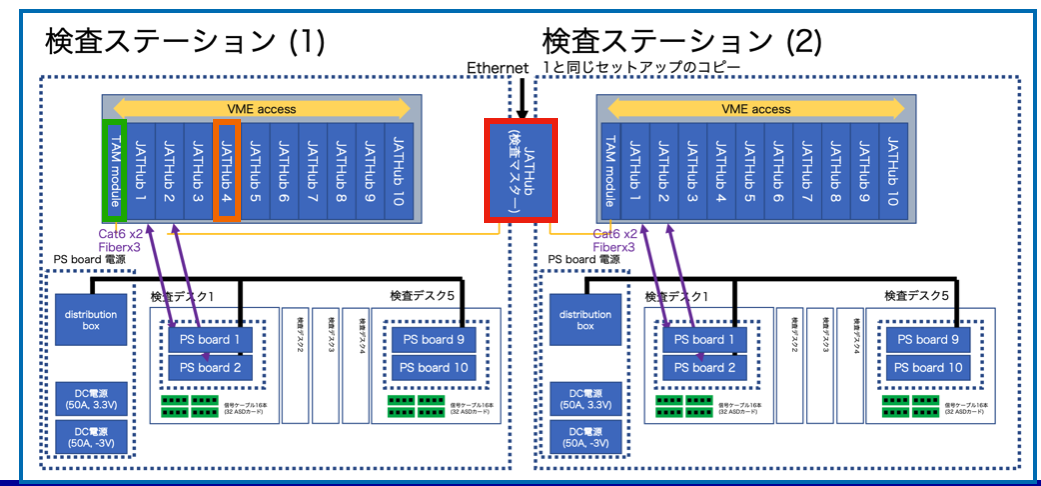
\includegraphics[width=16cm]{fig/QAQC/QAQCpararell.png}
\caption[並列化システムの概要]{並列化システムの概要}
\label{QAQCpararell}
\end{figure}
装した並列化システムの動作検証を東京大学で行なった(図\ref{QAQCpararellpicture})。すべての動作が期待通り動き、JATHubをマスターとしたPS boardの試験を行えることを検証した。

\begin{figure} 
\centering
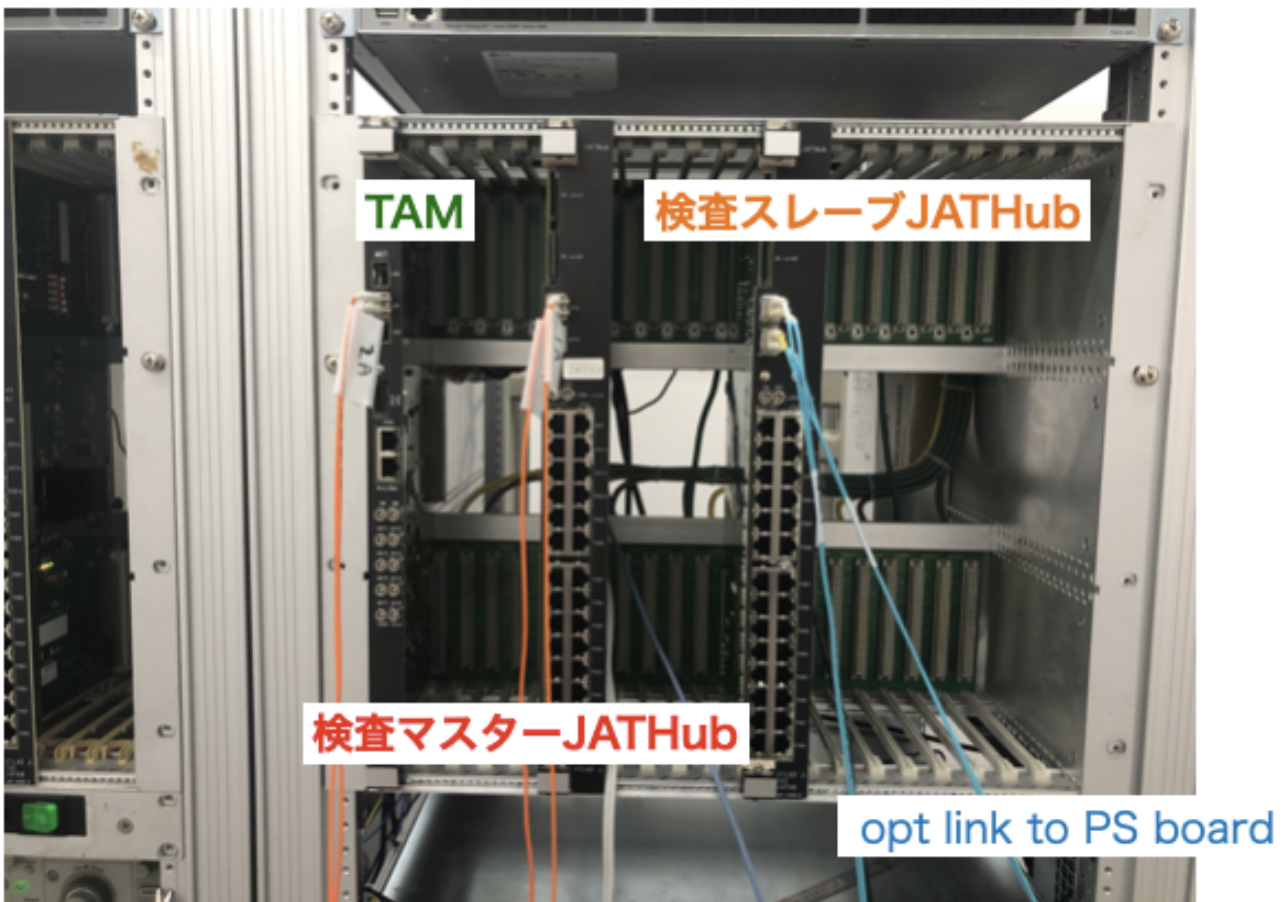
\includegraphics[width=16cm]{fig/QAQC/QAQCpararellpicture.png}
\caption[並列化システムの写真]{並列化システムの写真}
\label{QAQCpararellpicture}
\end{figure}

\subsection{コンパクトDAQシステムとしての応用例}
\label{subsec_compactdaq}
最後に本研究で開発したQAQC用JATHubの応用例について紹介する。本システムはデスクトップでも給電可能なコンパクトなDAQシステムであること、汎用的なOSであるUbuntuを搭載しており、ユーザーによる使い方のカスタマイズが容易であることからさまざまな応用が期待される。
実際に使用された例を2つ紹介する。1つ目の使用例はEIL4チェンバー検査試験である。そのときのセットアップを図\ref{JATHubEIL4}に示す。Phase2実験に向けて新たに開発されたEIL4チェンバーの各チャンネルのefficiencyを測定するため、JATHub、PS board、ASDを繋げたシステム利用している。QAQC用JATHubを拡張してセルフトリガー機構を実装し、宇宙線ミューオンに対する各チャンネルのefficiencyを測定している。
\vskip0.5\baselineskip(\ref{})

\begin{figure} 
\centering
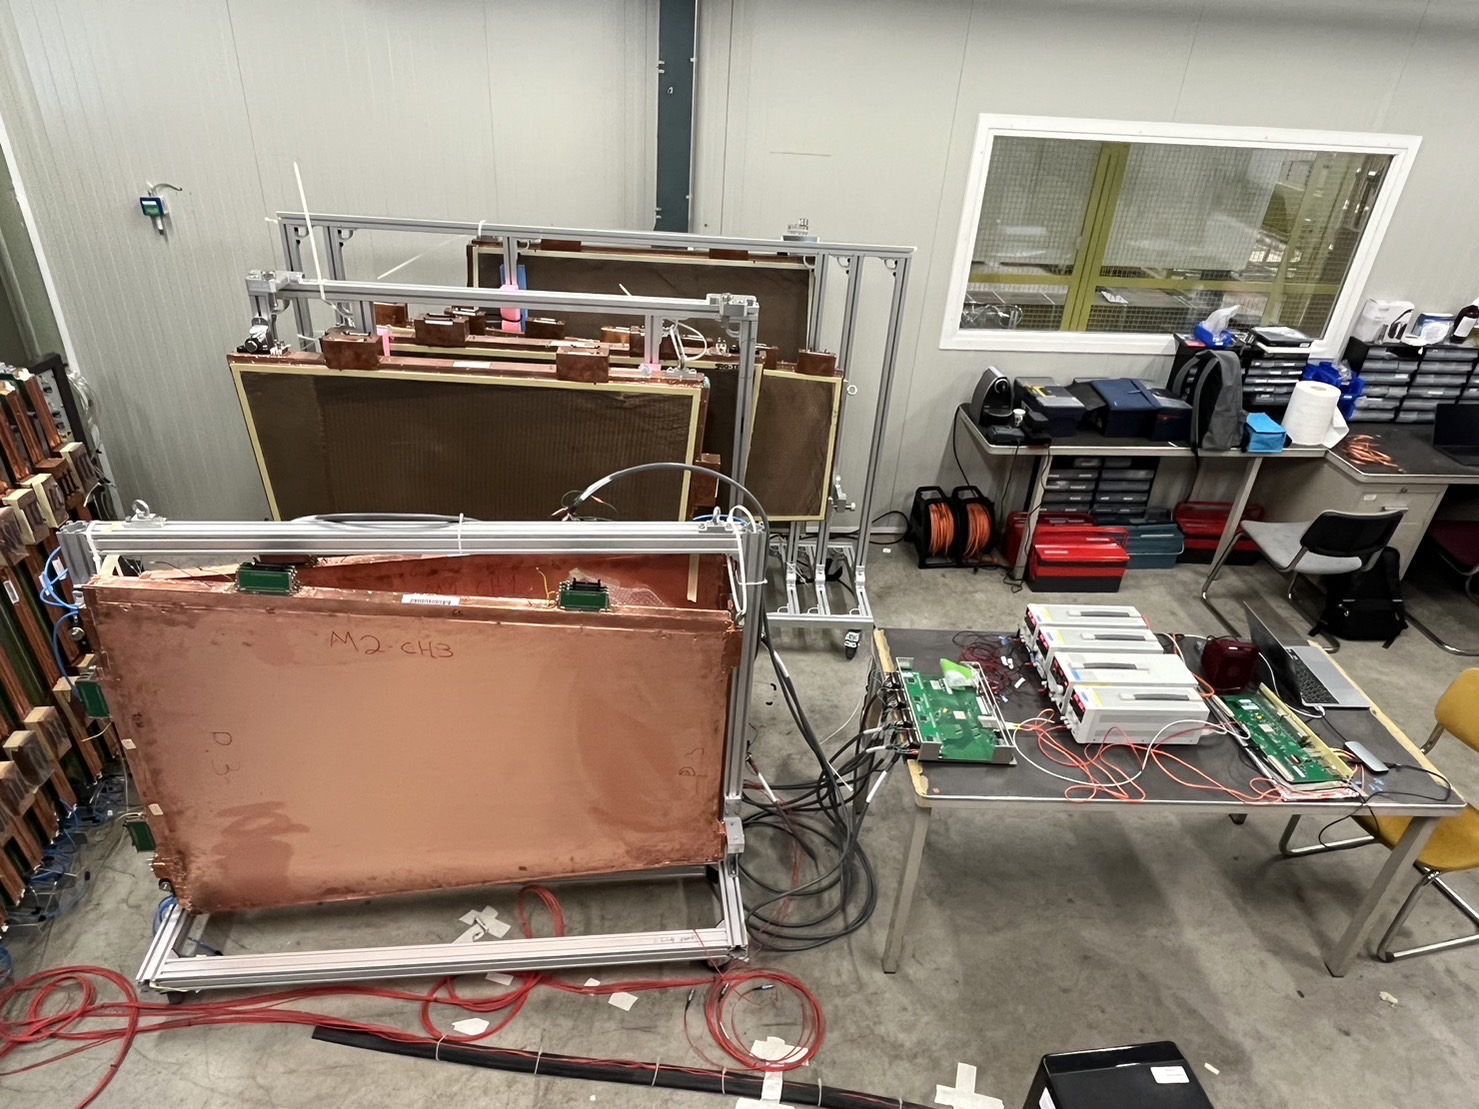
\includegraphics[width=16cm]{fig/QAQC/JATHubEIL4.JPG}
\caption[QAQC用JATHubの使用例:EIL4チェンバー試験]{QAQC用JATHubの使用例:EIL4チェンバー試験\cite{mt_wada}}
\label{JATHubEIL4}
\end{figure}

2つ目の例はPS baordのUX15における放射線耐性試験である(図\ref{JATHubSEU})。実際の実験中の放射線環境下におけるSEUの発生頻度を測定する試験である。この試験ではPS boardからSEUが発生するたびに光リンクを介してそれが知らされ、長時間にわたるSEUをモニターするために使われた。

\begin{figure} 
\centering
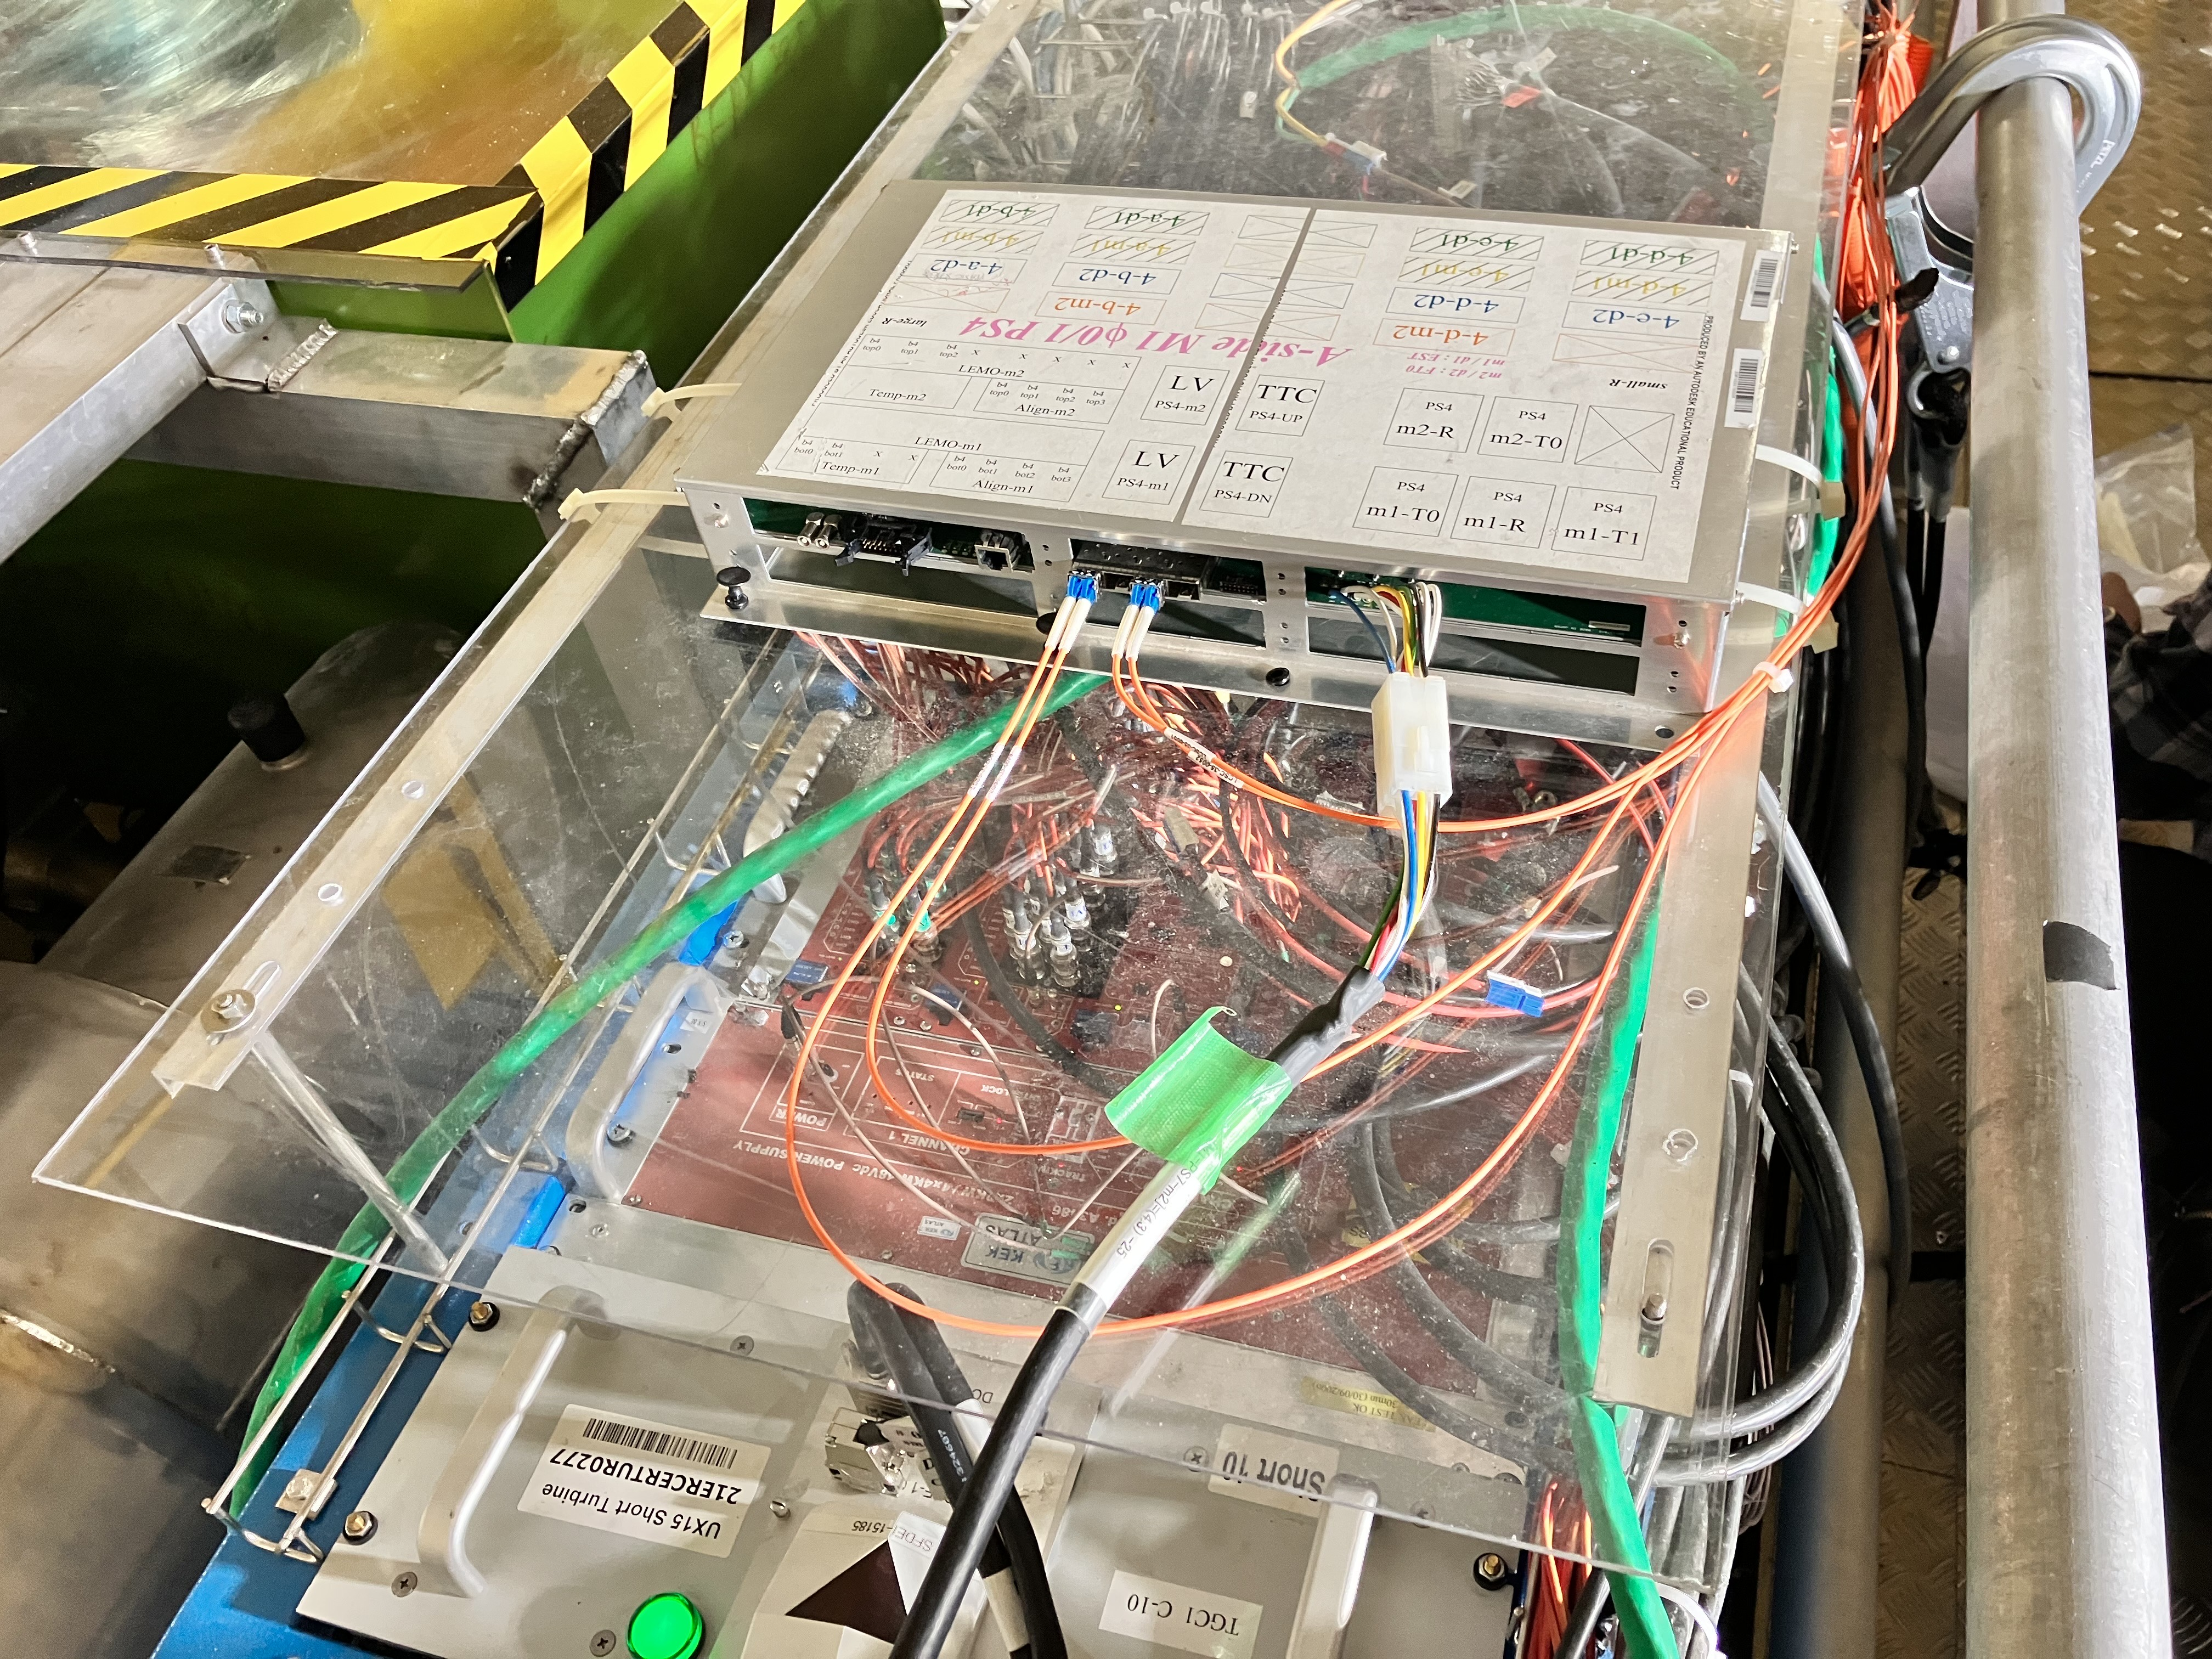
\includegraphics[width=16cm]{fig/QAQC/JATHubSEU.JPG}
\caption[QAQC用JATHubの使用例:PS board SEUモニター]{QAQC用JATHubの使用例:PS board SEUモニター\cite{mt_hashimoto}}
\label{JATHubSEU}
\end{figure}

そのほかにもそのコンパクトさと汎用性を以下してTAMモジュールのQAQC試験や、PS boardのメンテナンス目的でも本システムは利用されていく。。